\chapter{Estrutura e Materiais}

\section{Escopo}

\subsection{Número de Pessoas}

	A partir da análise de dados do IBGE\cite{2010IBGE} verificamos que a média do número de componentes das famílias brasileiras varia entre 3,2 a 3,6 pessoas por residência. Considerando que na definição do projeto pretendemos buscar que a casa seja versátil, podendo suportar visitas e um eventual aumento da família, arrendondamos os números do IBGE\cite{2010IBGE} para mais, definindo para 4 o número de componentes da família. 


\subsection{Local}

	O local escolhido para a casa sustentável foi o Jardim Botânico, 27a Região Administrativa do Distrito Federal. A escolha do Distrito Federal como local do projeto foi feita a partir de análises da média anual de radiação solar global diária do atlas solarmétrico do Brasil feito pela CEPEL, que indica que o estado do Distrito Federal se localiza em uma faixa de segundo maior índice de radiação solar dentro do Brasil, o que foi determinante para escolha do local, pois a energia proveniente do sol é uma das principais alternativas para a geração de energia da casa.
	
	Outro fator que foi levado em consideração para a escolha do DF, foi um ranking realizado pela ONU onde o estado está posicionado em um dos melhores lugares pelo IDHM, o que caracteriza melhor qualidade de vida no quesito educação, renda e expectativa de vida, se comparado ao restante dos estados brasileiros. Assim, delimitada a região do Distrito Federal, o Jardim Botânico foi escolhido por conter grandes lotes, com áreas que podem passar dos $1000\si{\meter}^{2}$\cite{2010Terracap} e áreas construidas acima de $250\si{\meter}^{2}$\cite{2014Codeplan}. O tamanho do lote foi priorizado na escolha da localidade pois grandes áreas são necessárias para a implantação de tecnologias sustentáveis, como painéis solares e turbinas eólicas.
	
	Outro fator que foi determinante para a escolha da localização foi a renda domiciliar da região, que no Jardim Botânico no ano de 2013 teve média de 18,51 salários mínimos\cite{2013SeplanCodeplan}. O projeto de uma casa sustentável engloba o uso de tecnologias inovadoras e de alto custo, assim, o projeto visa atender famílias de alta renda.

\newpage

\section{Planta da casa}

A planta tem que ser planejada para que fatores ambientais como vento, sol, frescor das plantas e outros, sejam melhores aproveitados de forma a proporcionar conforto para os moradores.

\subsection{Incidência Solar}

As estações do ano são causadas pela inclinação do eixo de rotação da Terra em relação ao eixo perpendicular ao plano definido pela órbita da Terra ( chamado de plano da eclíptica) 

\begin{figure}[H]
  \begin{center}
	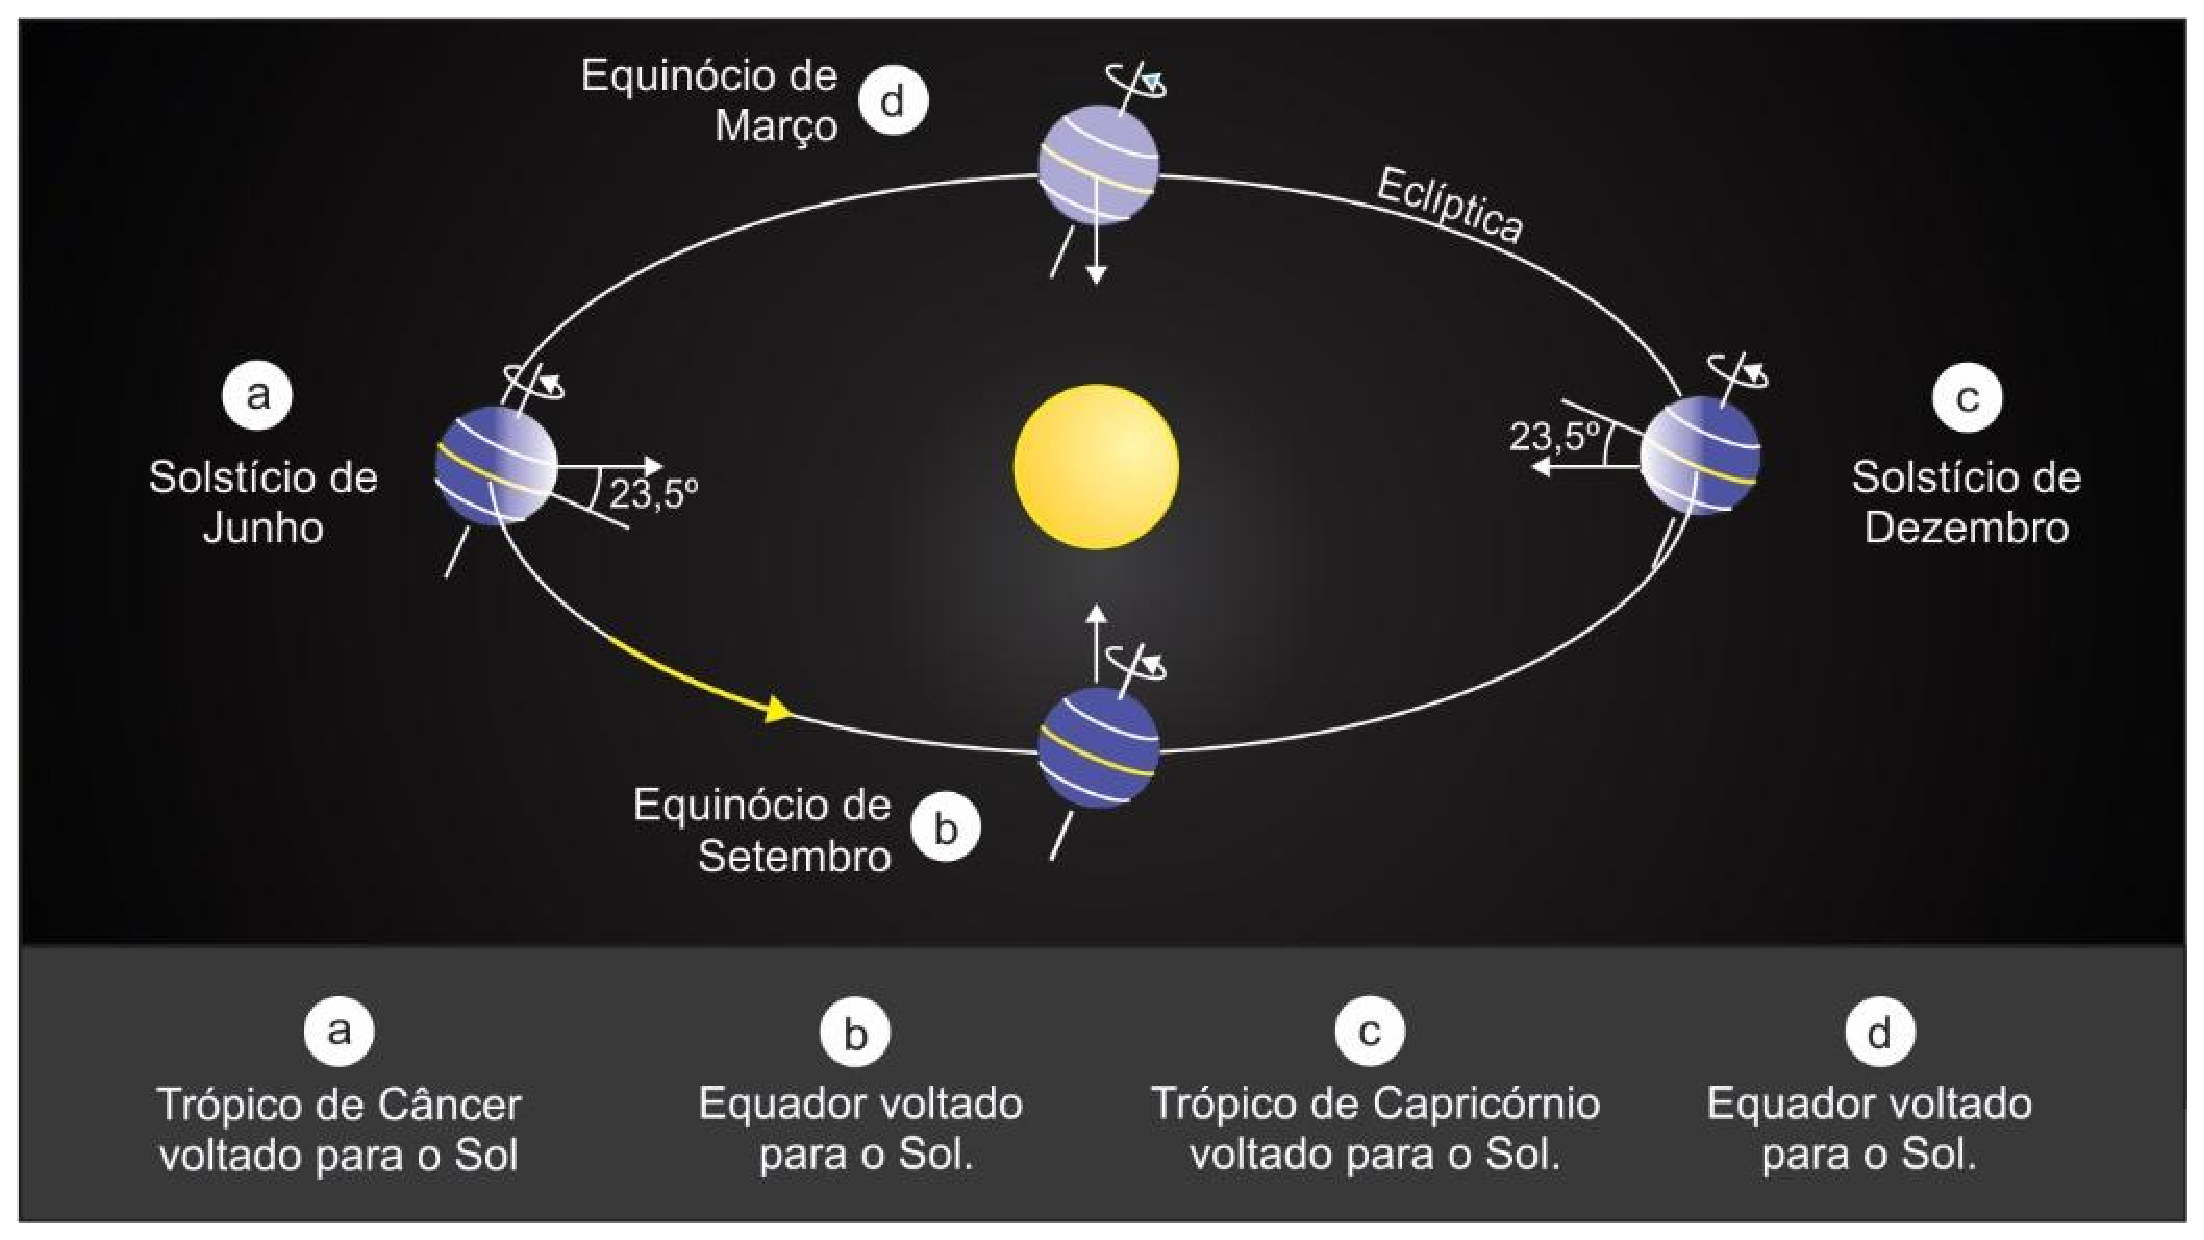
\includegraphics[keepaspectratio,scale=0.4,angle=0]{figuras/movimento.eps}
	\caption{Movimento da terra em torno do sol}
  \end{center}
\end{figure}

O Gnômon, haste vertical fincada perpendicularmente ao solo, é uma das formas de se observar a movimentação do Sol ao longo do ano. O tamanho da sombra formada pela haste depende da hora do dia e da época do ano.  através do gnômon, que é. Ao longo do ano, à mesma hora do dia, a sombra é máxima no solstício de inverno, e mínima no solstício de verão.

\begin{figure}[H]
  \begin{center}
	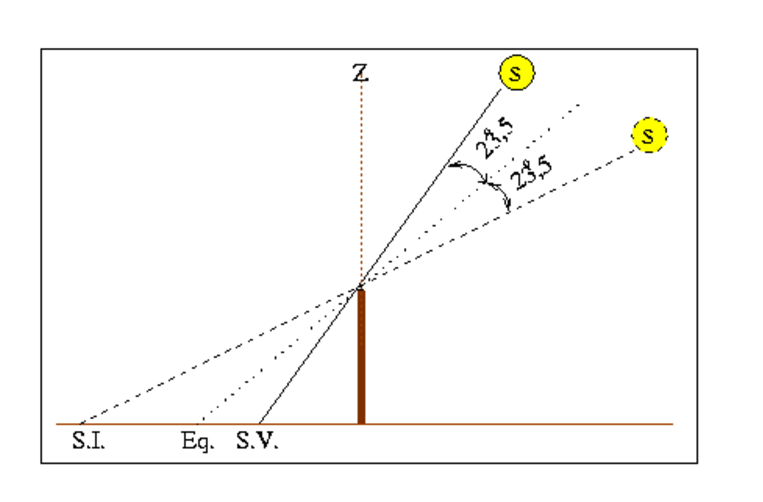
\includegraphics[keepaspectratio,scale=1,angle=0]{figuras/inclinacao.eps}
	\caption{Gnômon, S.I: Solstício de Inverno e S.V: Solstício de Verão
}
  \end{center}
\end{figure}

A partir do Gnomôn pode-se registrar numa Carta Solar a inclinação do sol conforme o horário e data, aplicável para uma linha de latitude correspondente, no caso de Brasília verifica-se a carta solar referente à latitude de aproximadamente 15°46’ Sul.

\begin{figure}[H]
  \begin{center}
	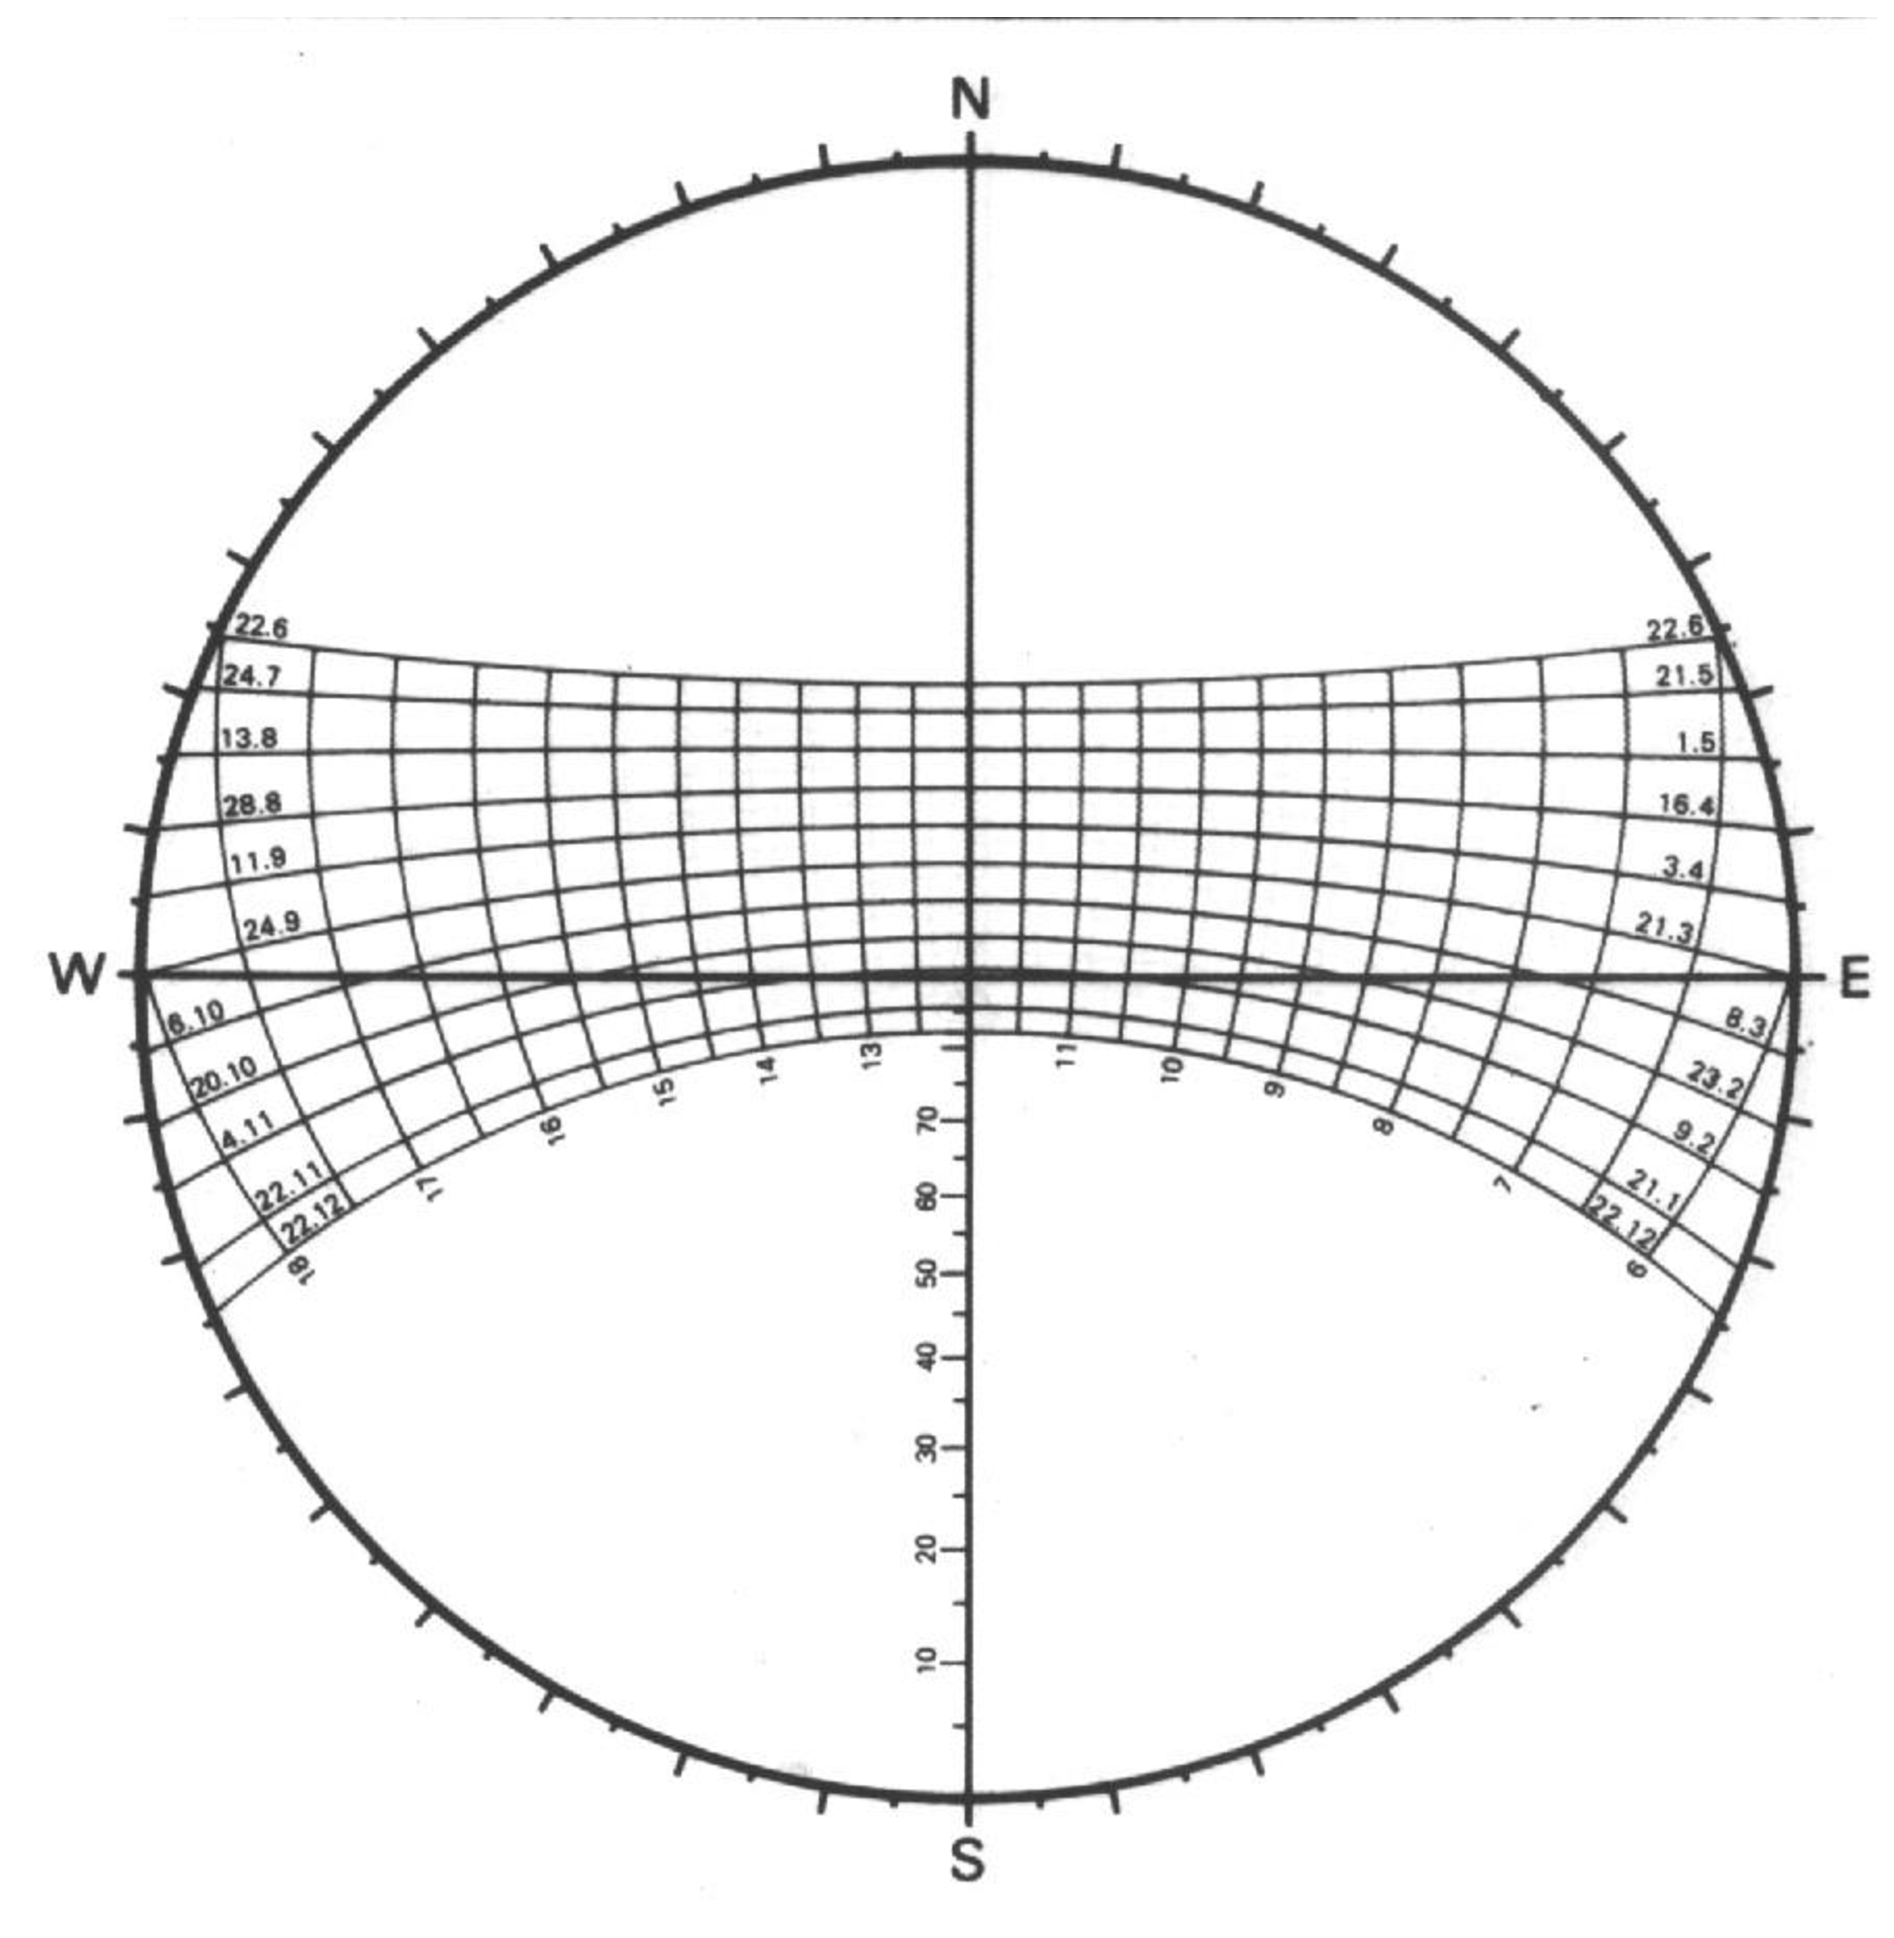
\includegraphics[keepaspectratio,scale=0.3,angle=0]{figuras/bioclimatico.eps}
	\caption{Carta solar de brasília. 
}
  \end{center}
\end{figure}

\subsection{Ventos}

	No decorrer da estação chuvosa os ventos predominam o quadrante Norte, com variação NW (Noroeste)  e NE (Nordeste), no período os ventos mais fortes vêm de NW. A partir do mês de março predominam os ventos de direção E (Leste). No período de estiagem aumenta a incidência dos ventos de Sul e Sudeste.

	A tabela \ref{direcao_ventos}\cite{2015Instituto} mostra a direção dos ventos durante todo o ano:

\begin{table}[H]
\begin{tabular}{|c|c|c|c|c|c|c|c|c|c|c|c|}
\hline 
Jan & Fev & Mar & Abr & Mai & Jun & Jul & Ago & Set & Out & Nov & Dez\tabularnewline
\hline 
\hline 
NW & E & E & E & E & E & E & E & E & NE & NW & NW\tabularnewline
\hline 
\end{tabular}
\caption{Direção dos ventos durante o ano}
\label{direcao_ventos}
\end{table}

\subsection{Planta}

	Analisando as necessidades do nosso projeto e da família para qual ele será construído, optamos por determinamos a nossa localidade no bairro Jardim Botânico, DF, e nos pautamos da média das casas desse setor e das famílias que lá residem para determinar a área útil da casa e a formação da família.

	Utilizamos como projeto base a planta baixa da “Casa Campo Grande”\cite{plantaCasa}, pois se mostra uma alternativa válida no quesito número de moradores e espaço disponível para construção, tendo $240\si{\meter}^{2}$ de área construída.

\begin{figure}[H]
  \begin{center}
	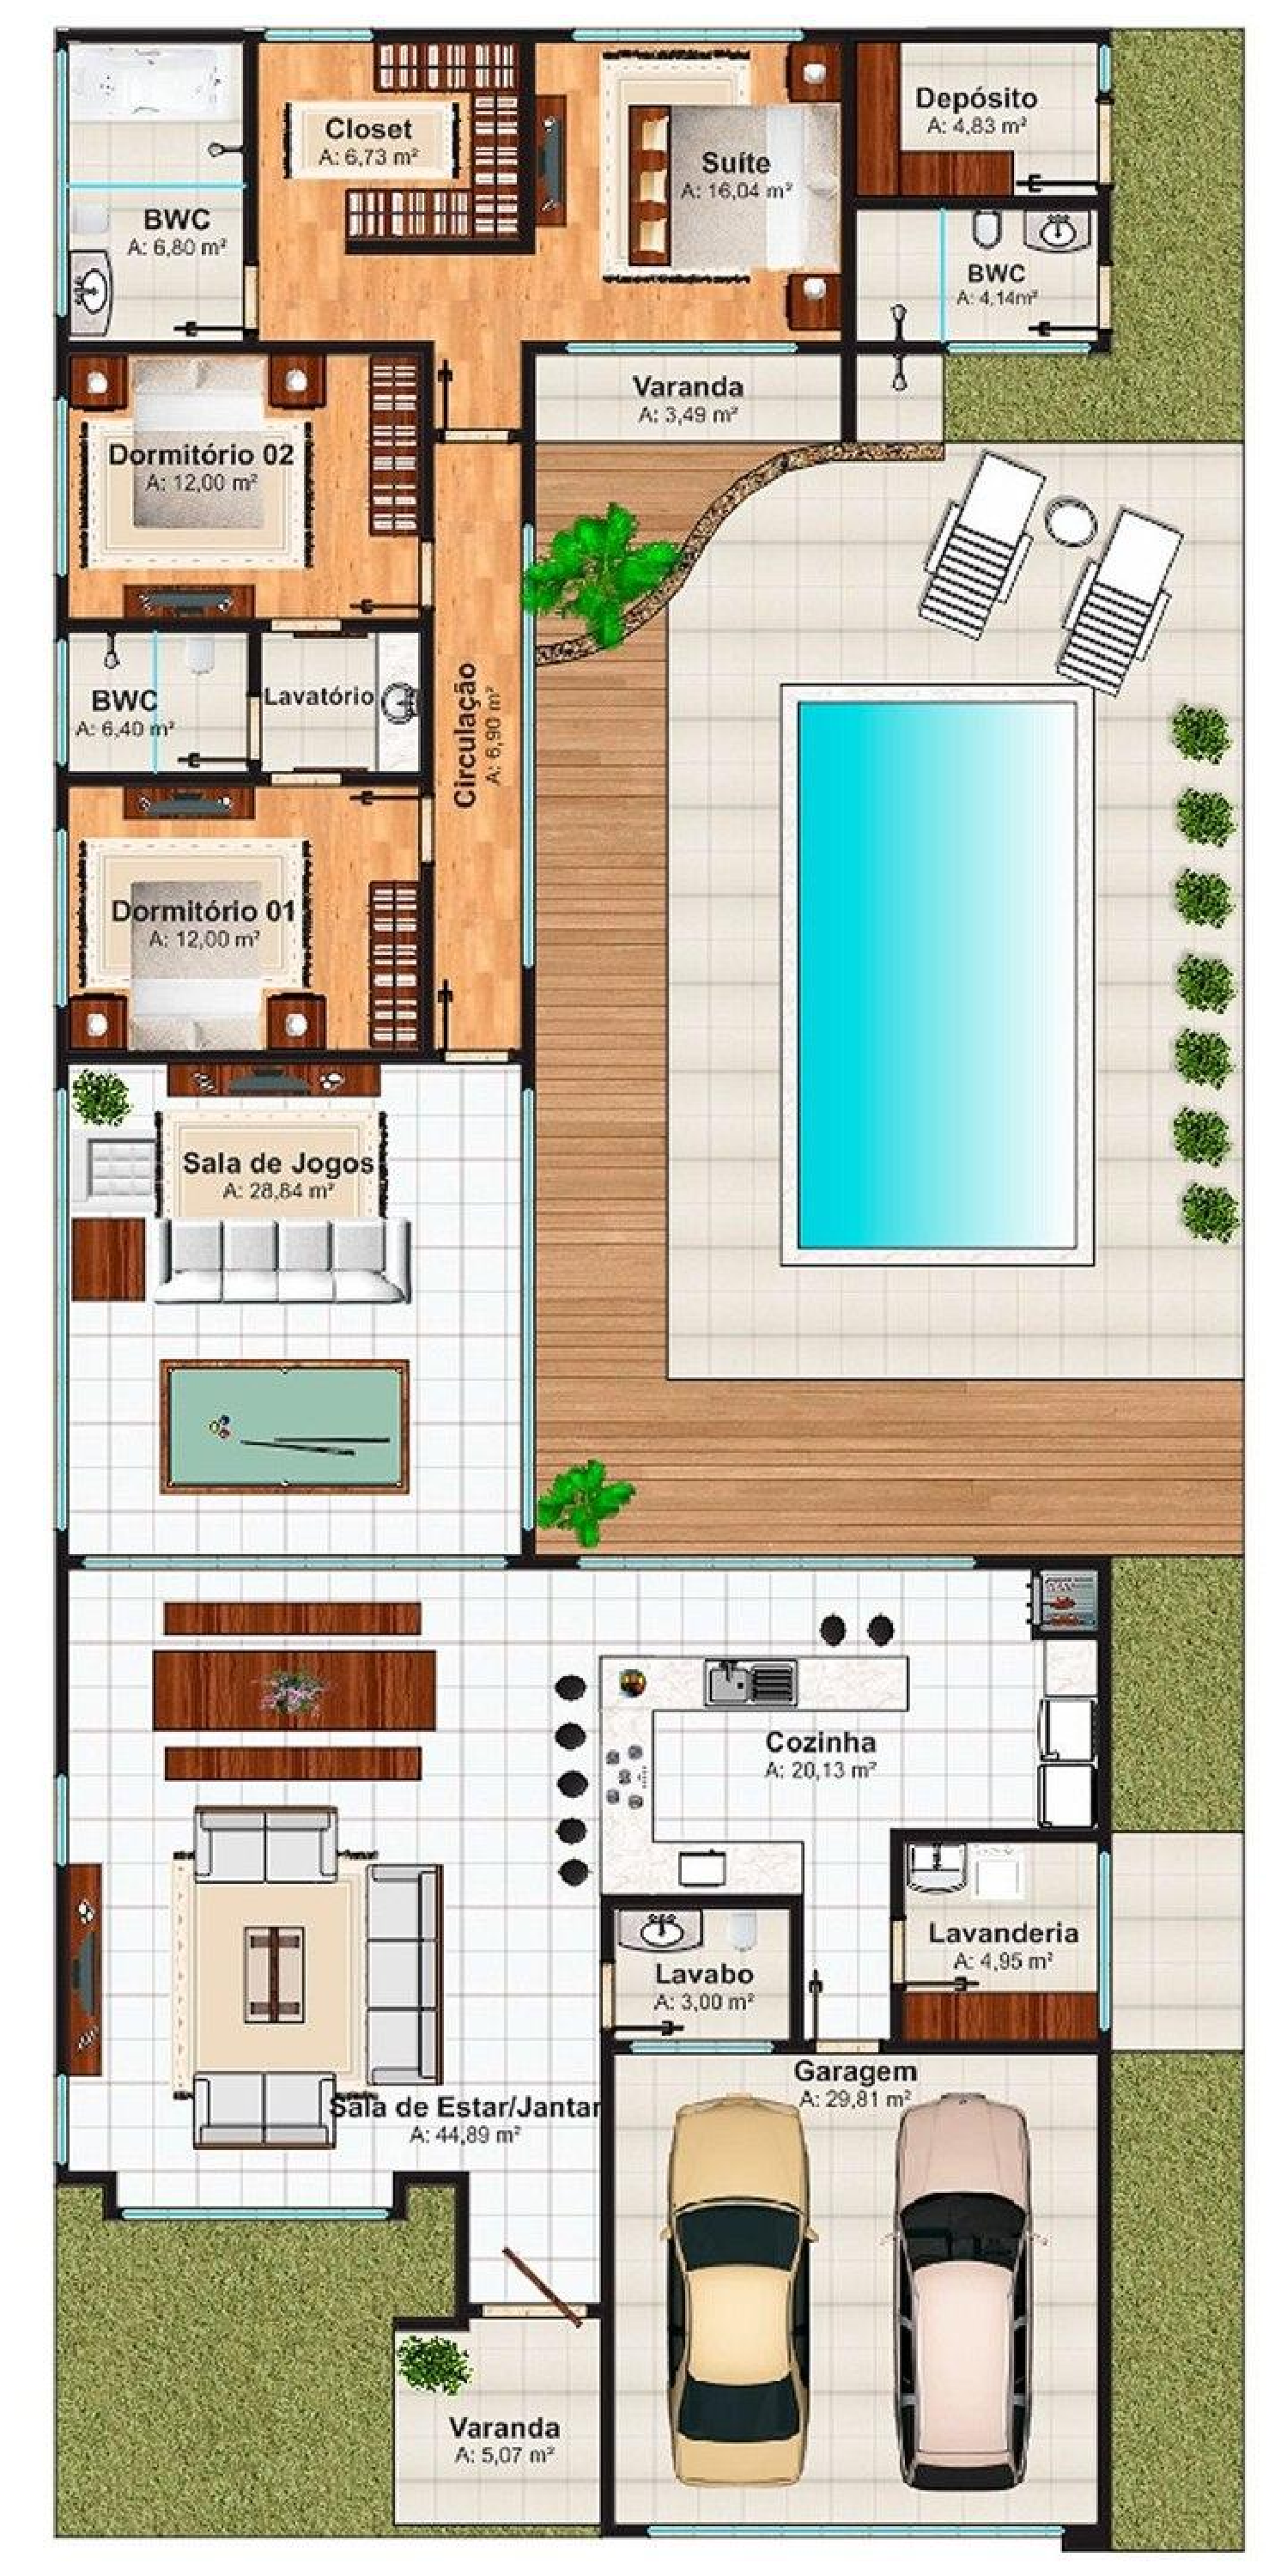
\includegraphics[keepaspectratio,scale=0.3,angle=90]{figuras/planta.eps}
	\caption{Planta da casa}
  \end{center}
\end{figure}


\begin{figure}[H]
  \begin{center}
	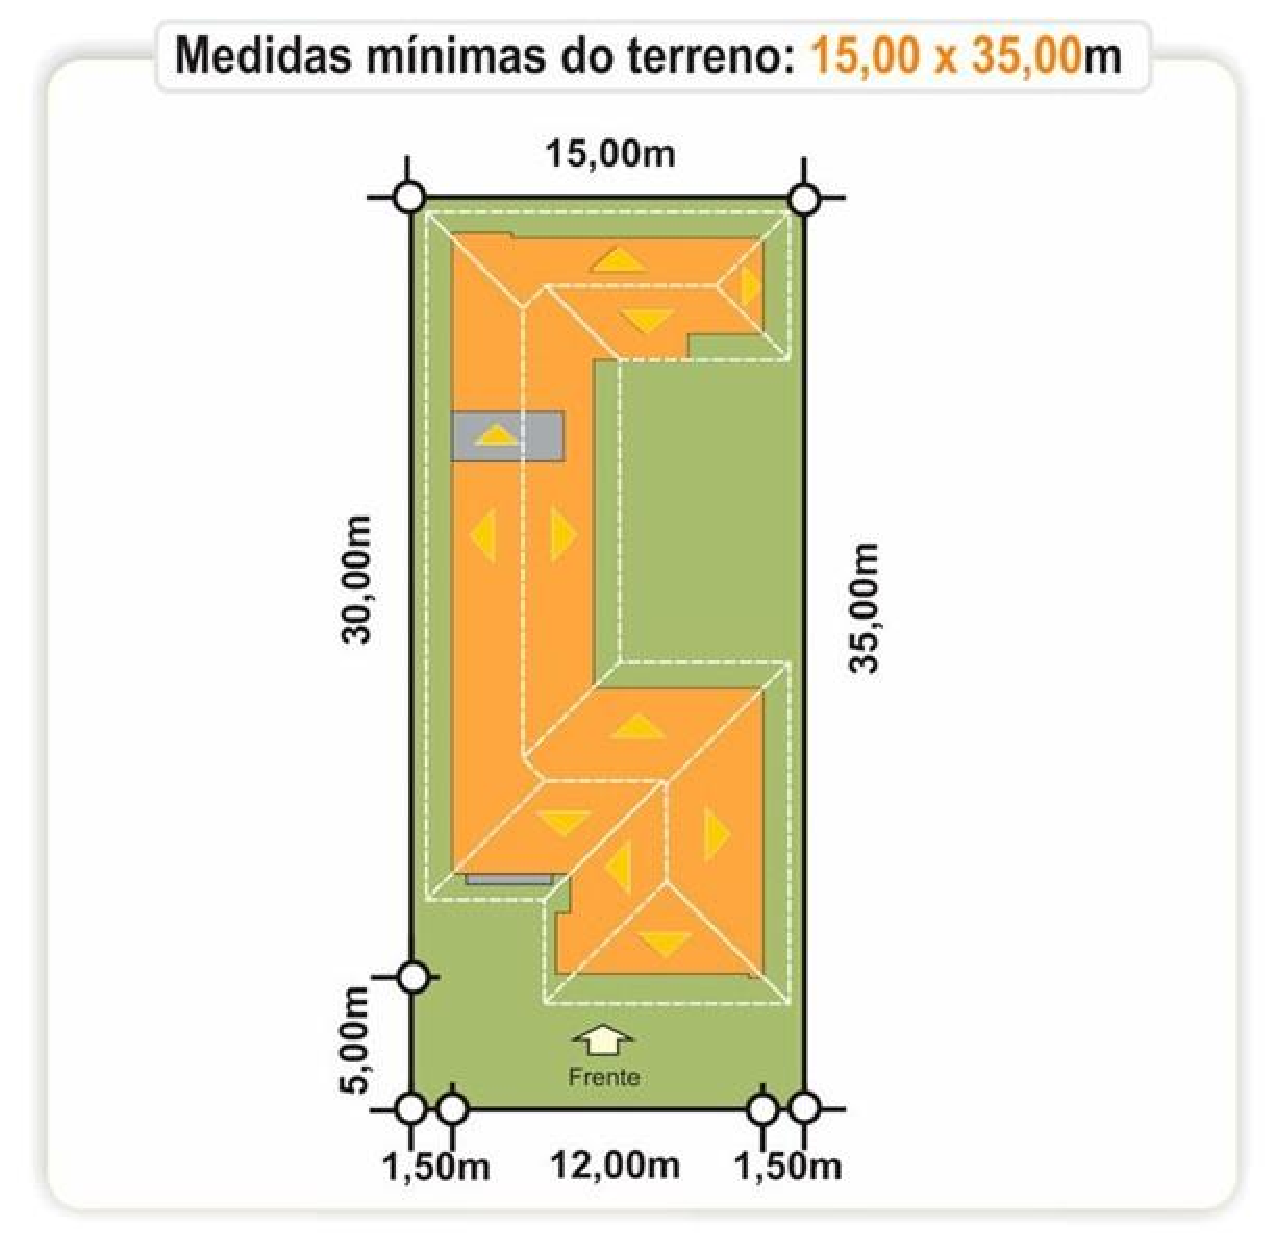
\includegraphics[keepaspectratio,scale=0.7,angle=0]{figuras/medidas.eps}
	\caption{Medidas da casa}
  \end{center}
\end{figure}

	Considerando as restrições do projeto base considerando as alterações feitas e aspectos de conforto térmico e maior eficiência das placas solares, determinou-se como possível localização da casa o Lote 3 do Conjunto N do Condomínio Jardim Botânico VI, de 15 metros de comprimento por 40 de largura, totalizando $600\si{\meter}^{2}$, sendo que a frente para a rua está posicionada para oeste.

\newpage

\begin{figure}[H]
  \begin{center}
	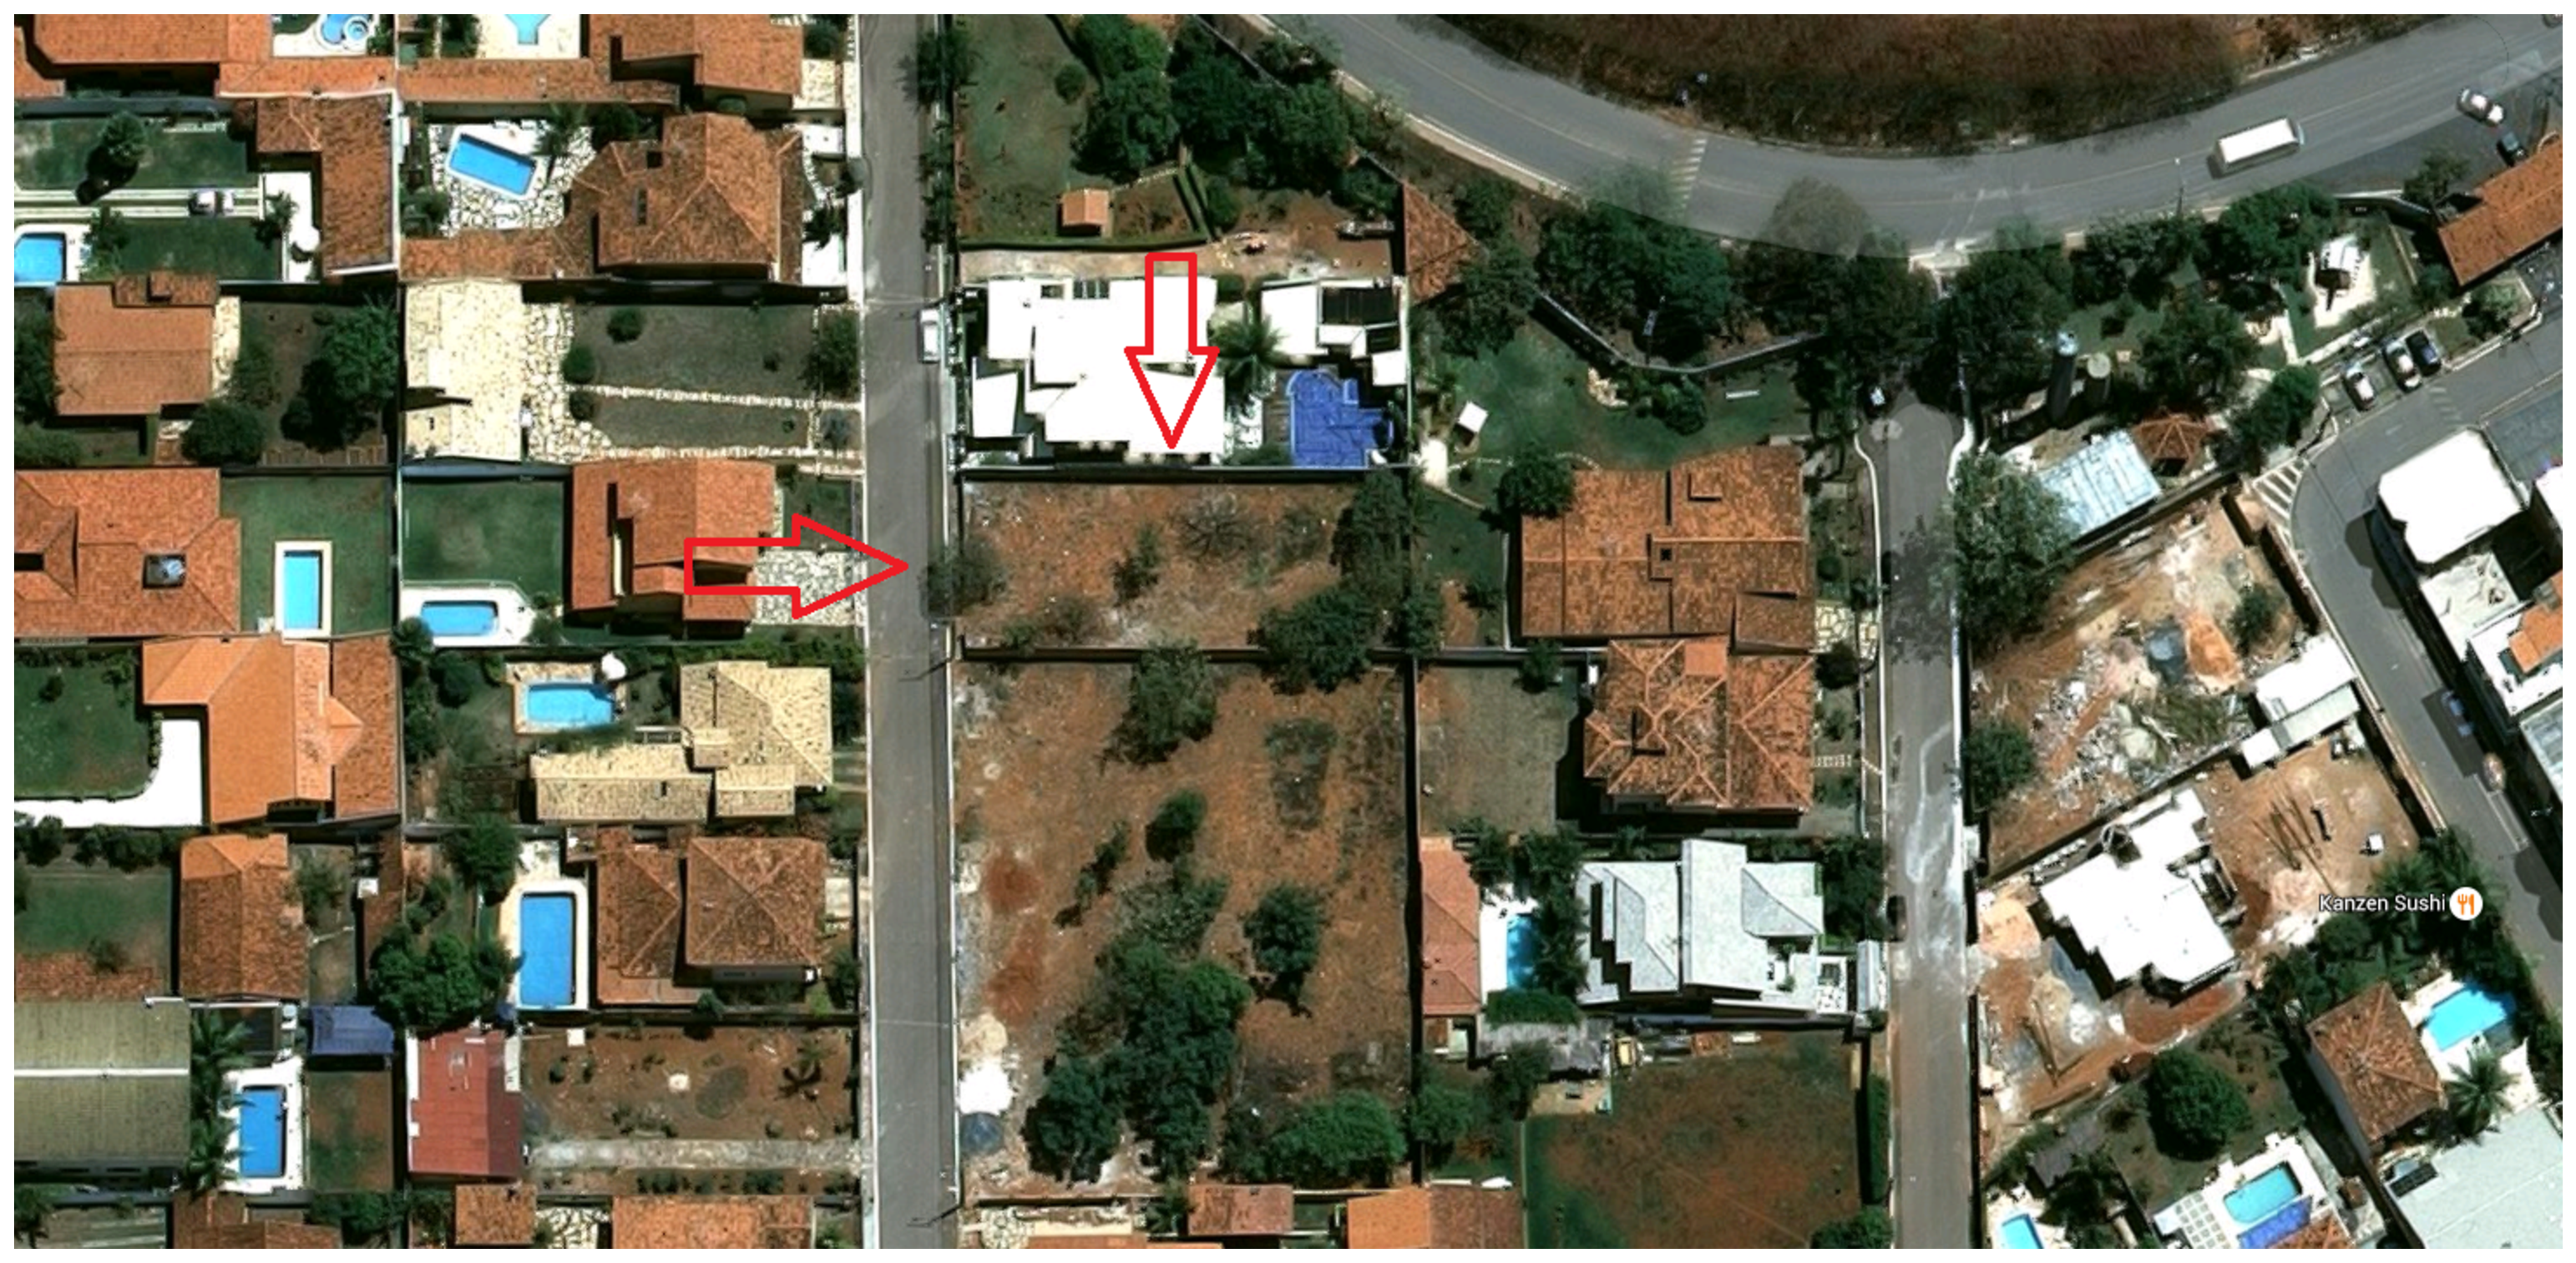
\includegraphics[keepaspectratio,scale=0.3,angle=0]{figuras/terreno.eps}
	\caption{Terreno da casa}
  \end{center}
\end{figure}

	O valor aproximado do metro quadrado de um lote no Jardim Botânico com base em valores do ultimo edital da Terracap\cite{TerracapJB} para dois lotes próximos da localidade escolhida. Para tanto, a média aritmética entre os valores por metro quadrado dos dois lotes foi calculada. 

$$\dfrac{292000}{802} = 364,09 \textup{ reais}/\si{\meter}^{2}$$
$$\dfrac{280000}{750} = 373,33 \textup{ reais}/\si{\meter}^{2}$$
$$\dfrac{364,09 + 373,33}{2} = 368,71 \textup{ reais}/\si{\meter}^{2}$$

Assim, o terreno escolhido com 600m² custa cerca de $R\$ 221.226,00$

\begin{figure}[H]
  \begin{center}
	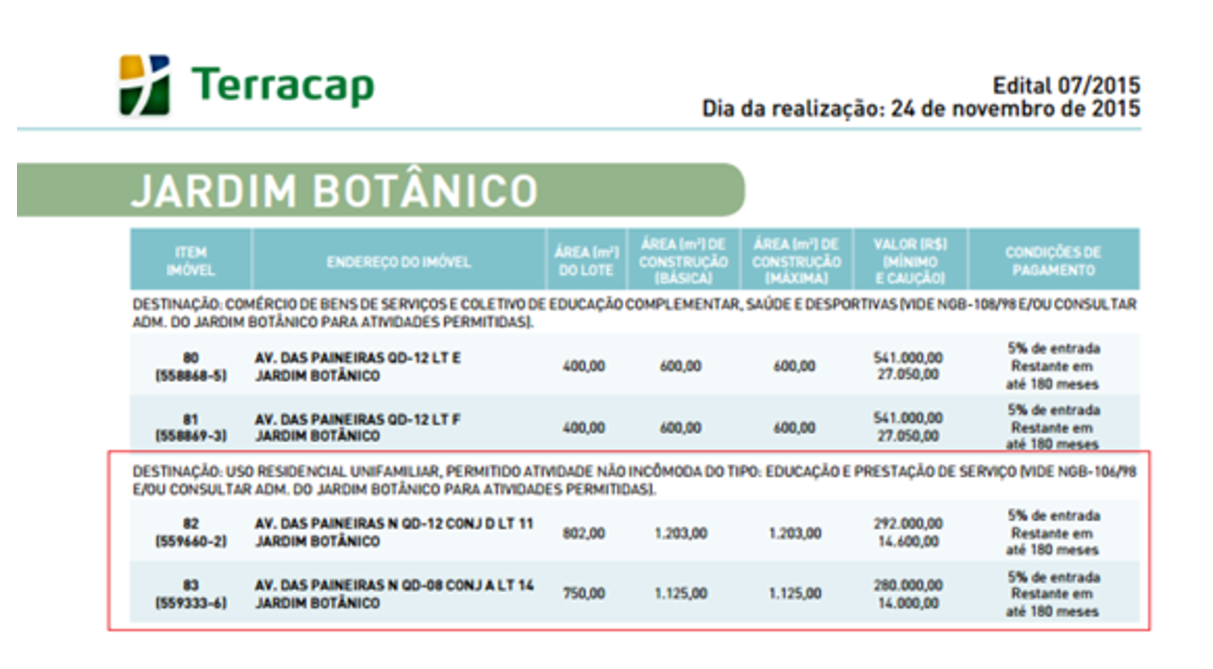
\includegraphics[keepaspectratio,scale=0.7,angle=0]{figuras/terracap.eps}
	\caption{Preço do lote}
  \end{center}
\end{figure}


\subsection{Justificativa da Planta}

	O formato da casa determina como e quanto será utilizado de materiais. No caso de uma casa sustentável visamos o menor impacto ambiental possível e maior economia de materiais, levando em consideração a segurança e resistência da casa. Na hora de fazer a planta, também nos preocupamos com fatores naturais como vento, chuva e o Sol, de forma com que a casa seja a mais arejada e iluminada possível.
	
	Na disposição de cômodos, o depósito é um espaço designado para automação da casa, onde irá ficar todas as máquinas que trabalham em conjunto para o bom funcionamento da casa. No canto superior esquerdo da planta, estão bem distribuídas as áreas nas quais os moradores poderão fazer suas necessidades físicas, que são 3 quartos, 3 banheiros e 1 closet. Mais abaixo, está uma área designada para a convivência social, não só dos integrantes da casa, mas também de suas visitas, salão de jogos, piscina e sala de estar. Também fizemos a parte onde serão feitas as atividades domésticas da casa, como cozinhar, lavar e  limpar. Estes cômodos estão bem distribuídos em cozinha, lavabo e lavanderia. Para finalizar, temos o espaço para a garagem e uma varanda. 

\begin{figure}[H]
  \begin{center}
	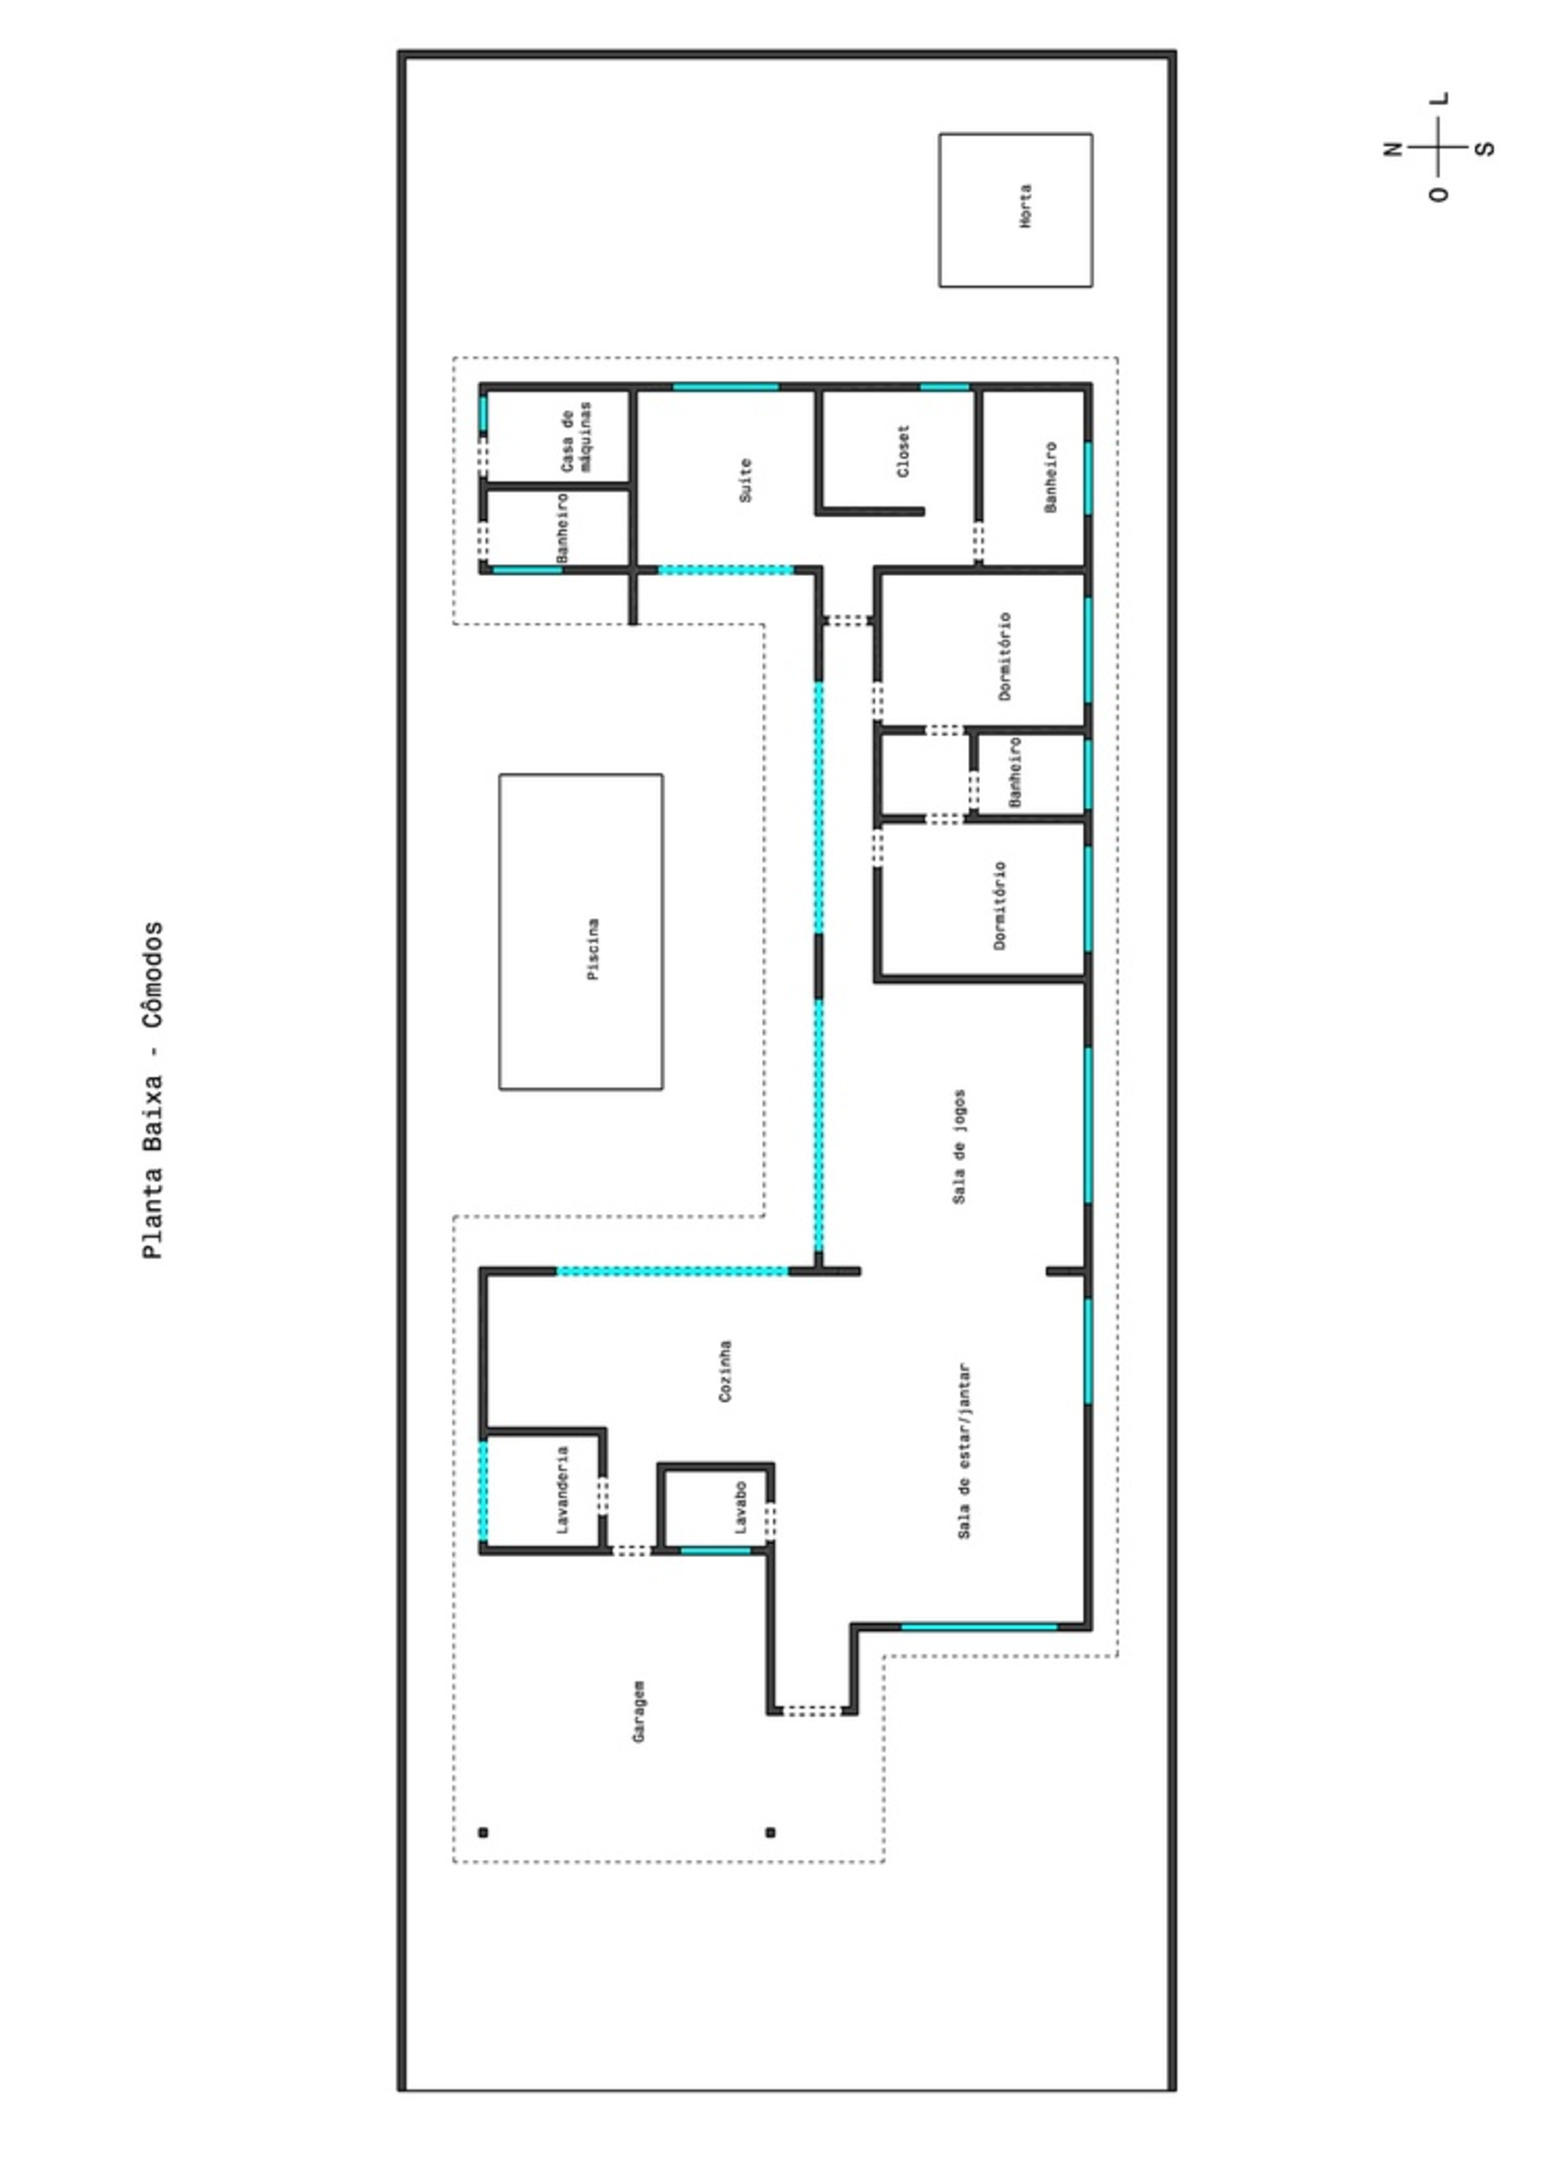
\includegraphics[keepaspectratio,scale=0.45,angle=270]{figuras/planta_comodos.eps}
	\caption{Planta baixa da casa com cômodos}
  \end{center}
\end{figure}

\begin{figure}[H]
  \begin{center}
	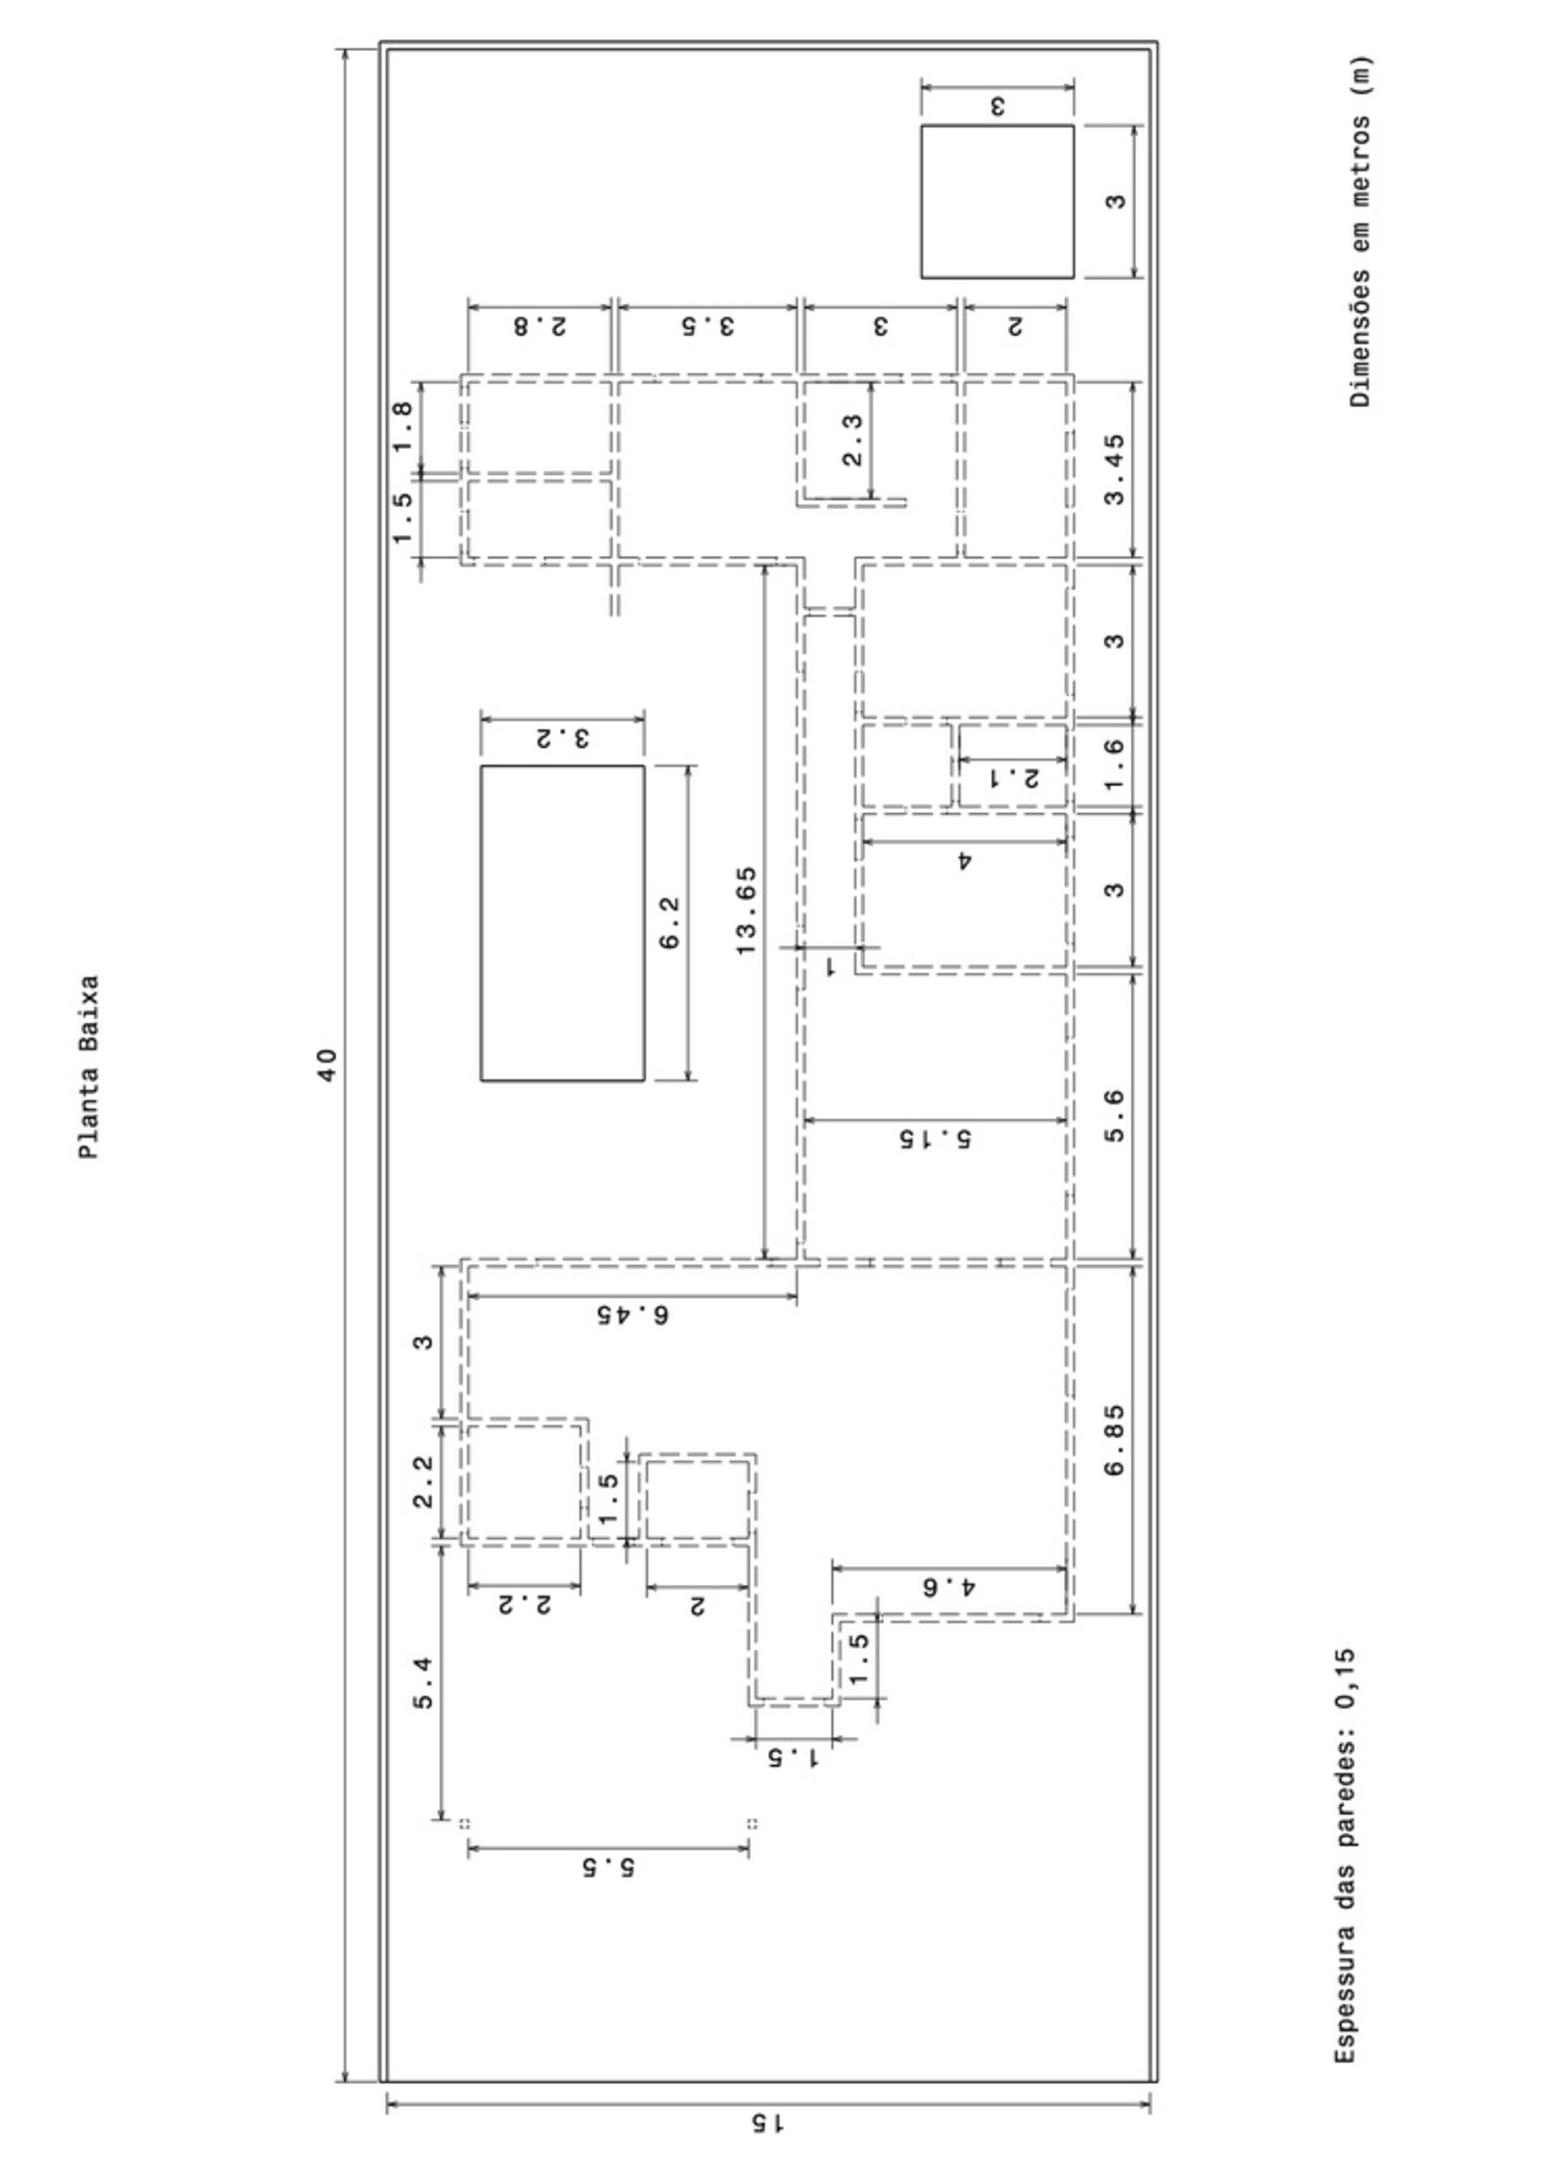
\includegraphics[keepaspectratio,scale=0.45,angle=270]{figuras/planta_baixa.eps}
	\caption{Planta baixa da casa}
  \end{center}
\end{figure}











\section{Materiais}

\subsection{Construção Sustentável}
	
	A construção sustentável é um processo produtivo que tende a realizar, no entorno, alteração conscientes, de forma a suprir as necessidades do uso do homem e de edificação, preservando os recursos naturais e o meio ambiente, garantindo para as gerações atuais e futuras uma qualidade de vida\cite{1992Baroni}. Para uma construção sustentável é necessário analisar o planejamento sustentável da obra, o aproveitamento passivo dos recursos naturais, a eficiência energética, a gestão e economia de água, a qualidade do ar e do ambiente interior, uso racional de materiais e o uso de produtos e tecnologias amigáveis ambientalmente\cite{2012Araujo}.


\section{Escolha dos Materiais Sustentáveis}

	Na escolha dos materiais devem ser consideradas a origem da matéria-prima, extração, processamento, gastos com energia para transformação, emissão de poluentes, biocompatibilidade, durabilidade, qualidade, entre outros que permitam classifica-los como sustentáveis ou ecológicos e elevar o padrão da obra no quesito de melhoria da qualidade de vida de seus habitantes e do próprio entorno. Essas características analisadas, devem estar de acordo com a geografia, tipologia, ecossistema, condições climáticas, resistência, responsabilidade social do ambiente onde será construído.

\subsection{Pisos - Ambiente Interno (Seco)}
	
	Caracteriza-se ambiente seco onde não há contato frequente com água, como sala de estar, quartos e escritório.

\subsubsection*{\textbf{Piso de bambu}}

	O processo de fabricação do bambu, em geral, é em linha, passando pelos cortes transversais e longitudinais, afim de colocar nas medidas padrões. Na sequência, o bambu passa por tratamentos físicos e químicos para a preservação do mesmo. Como as tiras de bambu são finas, o bambu passa por processos de prensagem e colagem para a formação das tábuas. E por fim, o acabamento por meio de lixamento, polimento e pintura.\cite{pisoBambu}

\subsubsection*{\textbf{Piso bambu X Outros pisos de madeira}}

     Em comparação com outras madeiras, o bambu tem crescimento muito rápido, com alta produtividade por hectare, além de ser altamente renovável e sustentável. O piso de bambu é mais forte, mais estável e mais durável do que a maioria dos pisos de outros tipos de madeira. Possui maior estabilidade dimensional e, portanto, menos expansão e contração do que pisos de madeiras tradicionais. A opção do piso de bambu traz um design à casa, o material está na moda no mercado e sua variedade de tonalidades que o próprio bambu tem aumenta o conforto do morador.



\subsubsection*{\textbf{Vantagens do bambu}}

	\begin{itemize}

		\item O bambu é relativamente forte e rígido

		\item O bambu pode ser cortado com ferramentas simples.

		\item A superfície do bambu é dura e limpa

		\item O bambu pode ser cultivado em pequena escala

		\item O retorno do capital é mais rápido do que se fosse usada madeira.

		\item As estruturas de bambu são flexíveis durante tormentas e terremotos

		\item O bambu pode ser usado com sucesso para reforçar um terreno deficiente, como por exemplo evitar desabamentos de terra ou para reforçar um caminho.
	\end{itemize}

\subsubsection*{\textbf{Desvantagens do bambu}}

	\begin{itemize}

		\item O bambu tem uma durabilidade natural baixa e necessita de tratamento

		\item O fogo representa um grande risco.

		\item Os talos do bambu não são totalmente retos, são estreitos. As emendas estão a distâncias diferentes e podem ser importunas quando se trabalha o material.

		\item A normalização é praticamente impossível devido à variação dos tamanhos.
	\end{itemize}

\subsubsection*{\textbf{Fábricas no Brasil}}

	\begin{itemize}

		\item \textbf{Ecori} -  São José do Rio Preto – SP – (17) 3222-2196

		\item \textbf{NeoBambu} - São Paulo – SP – (011) 5565-9029

		\item \textbf{Bambu Carbono Zero} - Campo Belo - SP - (11) 2803-7713

		\item \textbf{ParquetSP} - São Paulo - SP (11) 5053-8333

	\end{itemize}

	Empresa Escolhida
ParquetSP – A ParquetSP possui autorização para emissão de certificado FSC e Cerflor. Isso quer dizer que parte de seus produtos são provenientes de florestas manejadas e porque estão inseridos completamente em um processo denominado cadeia de custódia, ou seja, é um processo sistemático para rastrear produto da sua origem até o seu uso final.
Não há lojas em Brasília, logo a loja mais próxima e que obedece aos critérios de material ecológico e sustentável é a ParquetSP, localizada em São Paulo/SP.


\subsubsection*{\textbf{Preço}}

	O preço do metro quadrado, segundo a empresa, custa $R\$ 280,00$.


\subsection{Piso – Ambiente externo (Molhado)}

        Caracteriza-se ambiente molhado lugares que entram em contato com água frequentemente, como banheiros, área de serviços e áreas externas.

\subsubsection*{\textbf{Piso Cerâmico}}

	No processo industrial, as matérias-primas utilizadas, provenientes de jazidas próprias ou de terceiros, são estocadas no interior da fábrica. A dosagem de cada matéria-prima é feita segundo uma formulação percentual fornecida pelo laboratório, com base nos resultados obtidos em testes. Em seguida, o produto segue para o forno, onde é efetuada a queima da peça, é no forno onde o produto adquire suas características finais. Na saída de cada forno é realizado o processo de escolha, ou seja, o material que não está no padrão estabelecido volta para o início do processo. Na sequência o produto vai para a preparação de esmaltes e tintas, afim de melhorar a impermeabilidade, embelezar e aumentar a resistência ao desgaste. E por fim, antes da expedição, o produto passa pelo controle de qualidade, onde são analisadas amostras de cada lote de fabricação.\cite{pisoCeramico}

\subsubsection*{\textbf{Piso cerâmico X Outros pisos}}

O piso cerâmico é de fácil limpeza, ou seja, em ambientes com constante contato com água ele se torna mais fácil de secar e limpar, além de deixar o ambiente mais refrescado e aconchegante, pelo contrário dos pisos de cimento queimado e pisos de borracha, onde o excesso de água prejudica a conformidade dos mesmos. O piso cerâmico entra nos critérios escolhidos pois na sua fabricação, todos os resíduos gerados são reinseridos no processo de fabricação ou são matéria-prima para outros processos. O piso cerâmico vem  ganhando popularidade na decoração de casas nos últimos anos, pois estão disponíveis em uma enorme variedade de tamanhos e cores, assim como diferentes qualidades e preços. Ele é sem dúvida, um dos pisos mais versáteis, podendo ser utilizado em qualquer divisão da casa.


\subsubsection*{\textbf{Vantagens}}

	\begin{itemize}

		\item \textbf{Durabilidade}
		
		O piso cerâmico é muito mais durável que outro tipo de pisos. É também muito resistente à água e bactérias, sendo por isso uma boa opção para quem sofra de problemas respiratórios ou alergias. Devidamente instalado, o piso de cerâmica por durar por 20 anos ou até mais.

\newpage

		\item \textbf{Variedade de modelos}
		
		O piso cerâmico pode ser encontrado em diversas cores, desde as mais vibrantes aos tons mais sóbrios. Alguns modelos de pisos cerâmicos apresentam também textura ou imitam, inclusive, pisos considerados mais nobres, como madeira ou mármore. Como este tipo de piso é vendido à peça, é possível criar padrões elegantes ou mais originais, dependendo da forma como são dispostas as telhas no chão.

		\item \textbf{Isolamento}
		
		Em climas mais secos e quentes, o piso cerâmico ajuda a manter a temperatura ambiente mais fresca.

		\item \textbf{Preço}
		
		Uma vez que o piso cerâmico é mais durável, o seu valor é considerado um bom investimento face a outros tipos de piso mais caros.

		\item \textbf{Instalação}
		
		A própria de instalação também fica mais econômica, sendo também muito simples de ser feita.

		\item \textbf{Fácil manutenção}
		
		Este tipo de piso tem uma manutenção muito simples, para além de ser muito fácil de limpar. Para o manter bonito e nas melhores condições basta simplesmente varrer o chão, limpando de seguida com um esfregão úmido e um pouco de detergente doméstico suave.

	\end{itemize}

\subsubsection*{\textbf{Desvantagens}}

	\begin{itemize}

	\item \textbf{Isolamento}

	Embora o piso cerâmico seja ideal para climas mais quentes, visto dar frescura ao ambiente, em climas mais frios pode tornar-se demasiado gelado quando em contato com os pés.

	\item \textbf{Escorregadio}
	
	Quando molhado este tipo de piso pode levar a quedas e fraturas, uma vez que se torna muito escorregadio. É por isso aconselhável que esteja bem seco antes de alguém o pisar.

	\item \textbf{Delicado}
	
	Durante a sua instalação o piso cerâmico pode ser muito delicado, podendo inclusive partir-se com alguma facilidade, quando não são tidos todos os cuidados necessários para a sua correta colocação no chão.

	\item \textbf{Superfície dura}
	
	Ao contrário de outro tipo de pisos, como o piso em carpete, o piso cerâmico apresenta uma superfície muito dura. Em casas com crianças pequenas é aconselhável que se utilize tapetes nas zonas de maior passagem e brincadeiras, para que exista uma superfície mais fofa no caso de quedas.

	\end{itemize}

\subsubsection*{\textbf{Fábricas no Brasil}}

	\begin{itemize}

	\item \textbf{Itagres} - São Cristóvão - Tubarão – SC – (48) 3631- 2000


	\item \textbf{Portobello S.A.} - Tijucas - SC – Brasil – (48) 3279-2222 ou (61) 3361-0161

	\end{itemize}


\subsubsection*{\textbf{Empresa escolhida}}

Portobello S.A. – A Portobello produz anualmente 22,3 milhões de metros quadrados (m²) com 100\% de energia limpa, o gás natural. Ela recicla, reforma ou reutiliza 99,5\% de todo o resíduo sólido gerado no processo industrial. Mantém áreas equivalentes de preservação permanente para as áreas próprias de onde retiram a matéria-prima, sendo 291 hectares com preservação garantida. Reduziu de 5 para 3 anos o tempo de retorno das áreas exploradas para sua vocação natural através de um especial método de recuperação.
O descarte da água usada no processo industrial é zero graças à operação em circuito fechado que recicla a água em uma Estação de tratamento de efluentes para que seja novamente utilizada. E toda água utilizada nas ações não industriais vão para uma das 14 Estações de Tratamento de Água Doméstica e são devolvidas ao sistema pluvial em condições apropriadas.
A fabricante Portobello tem filiais em todo Brasil, e em Brasília se encontra nos seguintes endereços: SIA Trecho 03, Lote 550 – SUL e SEPN – Qd 509, Conj. B – Loja08/76 – Edifício Contag – Asa Norte.
A empresa escolhida está dentro dos critérios de material ecológico e sustentável estabelecidos no projeto.




\subsubsection*{\textbf{Preço}}
	
	O preço no mercado da cerâmica $48\times48 c\si{\meter}^{2}$ está entre $R\$ 27,90$ à $R\$ 34,90$.\cite{precoCeramica}


\subsubsection*{\textbf{Madeira Plástica Ecológica}}
	
A madeira plástica vem como uma opção sustentável para o uso da madeira em ambientes externos (decks, piers e outros). O produto é resultante de matérias-primas recicláveis, por exemplo resíduos plásticos industriais variados\cite{EcoCasa}. É totalmente reciclado e reciclável, além de ser composto de material completamente sustentável\cite{ReWood}. A madeira plástica é ideal para locais de piscina pois, apresenta todas as vantagens que o plástico em si tem: não é atacado por insetos ou fungos, não sofre ação de pragas nem roedores, é resistente a umidade, maresia e ao apodrecimento, podendo ser utilizada em todos os ambientes hostis à madeira tradicional, e não requer nenhum tipo de tratamento especial. Além disso, apresenta uma maior fixação relativamente a pregos e parafusos, não solta farpas e pode ser trabalhada com as mesmas ferramentas da madeira.


\subsubsection*{\textbf{Vantagens}}
	
	\begin{itemize}
		\item Zero de manutenção
		\item Totalmente feita de resíduos plásticos.
		\item Resistência à umidade;
		\item Resistência mecânica;
		\item Imunidade a pragas;
		\item Resistência à intempérie;
		\item Dispensa qualquer tipo de manutenção;
		\item Não degrada;
		\item Dispensa a pintura com vernizes e tintas.
	\end{itemize}

\subsubsection*{\textbf{Produtos que podem ser obtidos com o uso de madeira plástica}}
	
	\begin{itemize}
		\item Decks
		\item Bancos 
		\item Lixeiras para áreas externas
		\item Assoalhos
		\item Fachadas
		\item Pergolado
	\end{itemize}

\subsubsection*{\textbf{Fábricas no Brasil}}
	
	\begin{itemize}
		\item \textbf{Ecopex} - Jandira - SP, Brasil - (11) 4181 1103
		\item \textbf{In Brasil} - São Gabriel União da Vitória - Paraná - (42) 3522-1771
		\item \textbf{ReWood} - (11) 2402-4230
	\end{itemize}

\subsubsection*{\textbf{Empresa Escolhida}}

ReWood –A formulação dos produtos da ReWood é exclusiva e incomparável, já que utiliza plásticos e fibras 100\% reciclados e aditivos importados, que proporcionam extrema durabilidade, beleza, aderência e resistência ao sol e chuva, mantendo sua cor original por muito tempo sem que haja necessidade de qualquer manutenção. Localizada em Parque Santo Agostinho – Guarulhos/SP.

\subsubsection*{\textbf{Preço}}

	$R\$146,00$ à $R\$ 224,00$ cada metro quadrado, sem a necessidade de manutenção futura \cite{BlogReWood}.


\subsection{Paredes - Tijolo Ecológico }

\subsubsection*{\textbf{Solo-cimento}}
	
	Solo-cimento é o material obtido pela mistura de solo, cimento e água. O tijolo deste material é feito pela prensa, manual ou automatizada, dessa mistura. Após a prensa ele passa pela cura e secagem, não sendo necessária sua queima, que lançaria resíduos tóxicos no meio ambiente, enquanto no processo tradicional é feito a queima do tijolo logo após a saída da prensa. Portanto, no processo da queima no tijolo tradicional, há emissões de gases como Dióxido de Carbono (CO$_2$), Dióxido de Enxofre (SO$_2$), Monóxido de Carbono (CO), Gases Oxidantes, Óxidos Nitrogenados e Compostos de Chumbo, gases esses que contribuem para o aquecimento global e poluição do ar\cite{1980Portland}.\\

\subsubsection*{\textbf{Tijolo ecológico X Tijolo convencional}}
	O tempo de construção com o tijolo ecológico é muito menor, devido aos encaixes que favorecem o alinhamento da parede. A estrutura é mais segura pois as colunas são embutidas nos furos, e a sua carga de peso é melhor distribuídas. O tijolo ecológico tem uma durabilidade que chega a seis vezes maior que a dos tijolos convencionais, além de isolamento térmico e acústico gerados pelos furos no meio dos tijolos, que formam câmaras de ar e por fim as instalações hidráulicas e elétricas podem ser realizadas através dos furos. O tijolo ecológico entra nos critérios de escolha de materiais pela forma em que se é produzida, gerando menos resíduos e impactos ambientais na sua fabricação comparado com os tijolos convencionais.




\subsubsection*{\textbf{Vantagens do tijolo ecológico:}}
	
	\begin{itemize}
		\item Seu modelo de produção é por meio da prensa hidráulica ou eco manual, onde a pressão exercida é de 6 toneladas, tornando-o regular, com faces lisas e que proporcionam um encaixe perfeito, viabilizando assim uma maior precisão também no cálculo de tijolos necessários na obra;

		\item A utilização dos tijolos ecológicos evita a necessidade do uso de materiais como arame, madeira, pregos e folhas de parede pronta para a instalação da rede elétrica, hidráulica etc;

		\item Possui isolamento acústico e térmico, o que possibilita tanto o aquecimento como o resfriamento do ambiente de maneira natural;

		\item Reduz a umidade nas paredes;

		\item Além de aumentar a resistência da estrutura, facilita toda a construção, uma vez que seu molde permite o encaixe fácil e rápido, sem a necessidade de utilização de gesso ou azulejos;

		\item Diferentemente dos tijolos tradicionais, os ecológicos necessitam de pequenas quantidades de cimento, dentre outros.

	\end{itemize}

\subsubsection*{\textbf{Desvantagens}}

	\begin{itemize}

		\item Requer pedreiro qualificado, com conhecimento da técnica de aplicação;

		\item Apesar de funcionar perfeitamente bem em climas secos, os tijolos ecológicos, quando aplicados em locais de climas úmidos ou de maior exposição à umidade, ainda não é totalmente indicado.

	\end{itemize}

\subsubsection*{\textbf{Fábricas no Brasil}}

	\begin{itemize}

		\item \textbf{Monteiro Tijolos} – Salto – SP – (11) 8649-9226

		\item \textbf{TerraMax} – Lagoa Santa – Belo Horizonte – MG – (31) 3371-8690

		\item \textbf{Tijoleko} – Anápolis – DF – (62) 8597-4998


	\end{itemize}

\subsubsection*{\textbf{Empresa esolhida}}
	
	Tijoleko - A matéria prima da empresa Tijoleko é cuidadosamente selecionada na jazida e periodicamente testada em laboratório. Além de seguir os critérios estabelecidos, localizado em Anápolis – GO.


\subsubsection*{\textbf{Preço}}

	Nas medidas de $25 cm \times 12,5 cm$ e $7 cm$ de altura, segundo a empresa, varia entre $R\$ 0,92$ à $R\$ 1,20$ a unidade.


\subsection{Tinta Mineral Natural}

	
	Conhecida também como tinta mineral ecológica, é feita na base de terra crua, emulsão aquosa e cargas minerais para coloração específica. Tal matéria prima é retirada de jazidas certificadas e possui a opção de revestimento (pintura externa) tanto quanto tinta para interiores. \cite{EcoCasa}.

\subsubsection*{\textbf{Vantagens}}
	
	\begin{itemize}

		\item Não agride o meio ambiente

	As tintas minerais naturais são não tóxicas, e não prejudicam o meio   ambiente. Além disso, seu preparo e confecção e processo produtivo configuram fatores ecologicamente corretos.

		\item Não possui nenhum tipo de Composto Orgânico Volátil (COVs – reconhecido como um perigoso poluente)

	Os COVs são nocivos para o meio ambiente. Sua evaporação agride a camada de ozônio.Os produtos que contém esses compostos afetam a saúde, pois sua evaporação pode provocar problemas como irritação nas vias respiratórias, fadiga, falta de ar, dor de cabeça, náuseas, danos ao sistema nervoso, ao fígado, aos rins e câncer.
 
		\item Não possui biocidas, estabilizantes ou corantes
		
		\item Durável
		
		\item Lavável
		
		\item Contribui na manutenção de umidade relativa do ar e troca de calor
		
		\item Fácil aplicação e ótimo rendimento, dispensando qualquer base de preparo
 
	\end{itemize}

\subsubsection*{\textbf{Fábricas no Brasil}}

	\begin{itemize}

		\item \textbf{Solum} - Vila Madalena – SP,  Brasil -  (11) 3097-8716 

		\item \textbf{Kroten} - Pomerode - SC - Brasil - (47) 3395-0230 

	\end{itemize}

\subsubsection*{\textbf{Empresa Escolhida}} 

	Solum - Vila Madalena – SP. Em 2008 o Prêmio Planeta Casa concedeu à empresa o prêmio de Inovação em Materiais de Construção. O Mercado reconheceu o produto como um Revestimento de Terra Crua e Sustentável.  

\subsubsection*{\textbf{Preço}}

	Preço do balde de 18 litros = $R\$ 315,00$


\subsection{Telhado}

\subsubsection*{\textbf{Telha Ecológica}}

	Produzidas a partir de fibras naturais ou materiais reciclados, As telhas ecológicas apresentam baixo custo de produção e podem ser utilizadas com as mesmas aplicações das telhas convencionais.
	O processo de fabricação é baseado principalmente na fusão do material sob pressão e posteriormente o resfriamento. Primeiramente, o material é triturado em fragmentos pequenos, pois a redução de tamanho facilita sua fusão. Após da trituração, todo o material é depositado em formas e essas são colocadas em prensas, onde são levadas a temperaturas entre 160 e 200ºC. Após esse processo de fusão, o material é levado para o resfriamento em formas no formato tradicional de telha.\cite{D.C.Araujo}

\subsubsection*{\textbf{Telhas ecológicas X Outros tipos de telhas}}
Entre os diversos tipos de telha, sobressaem duas: a telha de cerâmica e a telha ecológica. Os produtos feitos de cerâmica, tem vantagens por sua produção reaproveitar os produtos não conformes, reduzindo os resíduos, e o uso de água e argila. Já as telhas ecológicas, feitas a partir de caixas de leite longa vida foi escolhido pois, ele é feito a partir de material reciclável, ou seja, o destino final de uma caixa de leite longa vida não é mais um aterro sanitário ou lixão, e sim matéria-prima para a fabricação de telhas ecológicas.



\subsubsection*{\textbf{Vantagens}}

	\begin{itemize}

		\item Fácil manuseio e instalação: seu estoque e transporte são fáceis (pois a telha é flexível) e reduzem o número de quebras / perda de material (é recomendado que seja utilizada mão-de-obra especializada);
		\item Economia de tempo e material: a maioria é mais leve que a telha tradicional, reduzindo os custos da construção (a estrutura é mais leve e o serviço é realizado rapidamente). É importante destacar que o planejamento é essencial para a redução dos custos, ou seja, o desenvolvimento de um bom projeto arquitetônico e estrutural é essencial, decidindo quais materiais e acabamentos serão utilizados antes mesmo de iniciar a obra;
		\item É um material resistente: são resistentes e flexíveis, resistindo a chuvas de granizo;
		\item A maioria não propaga chamas;
		\item São impermeáveis: absorvem muito menos água do que as telhas convencionais e geralmente seu acabamento evita a proliferação de limo;
		\item Promovem o conforto térmico: alguns tipos ajudam a criar um ambiente interno mais confortável (menos quente);
		\item Design: é possível encontrá-las em vários formatos e cores (inclusive pigmentada dos dois lados permitindo ser instalada sem forro). Além disso é possível pintá-las com tintas à base de água;
		\item São sustentáveis: geralmente produzidas com fibras e resinas, materiais reciclados (como papel, caixa de leite longa vida) e não contém amianto (o qual é tóxico);
	
	\end{itemize}

\subsubsection*{\textbf{Fábricas no Brasil}}
	
	\begin{itemize}
	
		\item \textbf{GLZ} - Telhas e Laminados Ecológicos - Santa Cruz do Sul - RS - (51) 8119-8393

		\item \textbf{Eccoclean Telhas Ecológicas} - Saquarema - RJ - (22) 2653-2531

		\item \textbf{ECO-LÓGICA} - Vicente Pires/DF - (61) 3034-0506
	\end{itemize}

\subsubsection*{\textbf{Empresa escolhida}}
	Eco-lógica – A empresa Eco-lógica tem sua sede na Chácara 167 – Lote 3A – Vila São José- Vicente Pires/DF. A Eco-lógica, é uma pequena empresa que vem aumentando seus lucros a partir da reciclagem das embalagens longa vida. A empresa escolhida entra nos critérios estabelecidos de material ecológico e sustentável.

\subsubsection*{\textbf{Preço}}

	Nas medidas $2,20\si{\meter} \times 0,90\si{\meter} \times 6\si{\meter\meter}$ a $R\$ 45,00 $.\cite{ecologica}


\subsection{Telhado}

Segundo um dos fabricantes\cite{2013Onduline}, a inclinação para maior conforto térmico é de 27\%, o que corresponde a aproximadamente $15,66^o$ de inclinação. Esta inclinação converge com a inclinação ótima para a obtenção de energia por meio das placas fotovoltáicas, cuja inclinação com face norte deve corresponder à da latitude para maior eficiência\cite{2013Portal}. Portanto conclui-se que $15^o$ de inclinação com a face voltada para o Norte privilegia a captação de energia solar ao mesmo tempo que atende aos requisitos da Telha Ecológica.

A partir destas especificações foi elaborada uma renderização 3D da casa.
\newpage

\begin{figure}[H]
  \begin{center}
	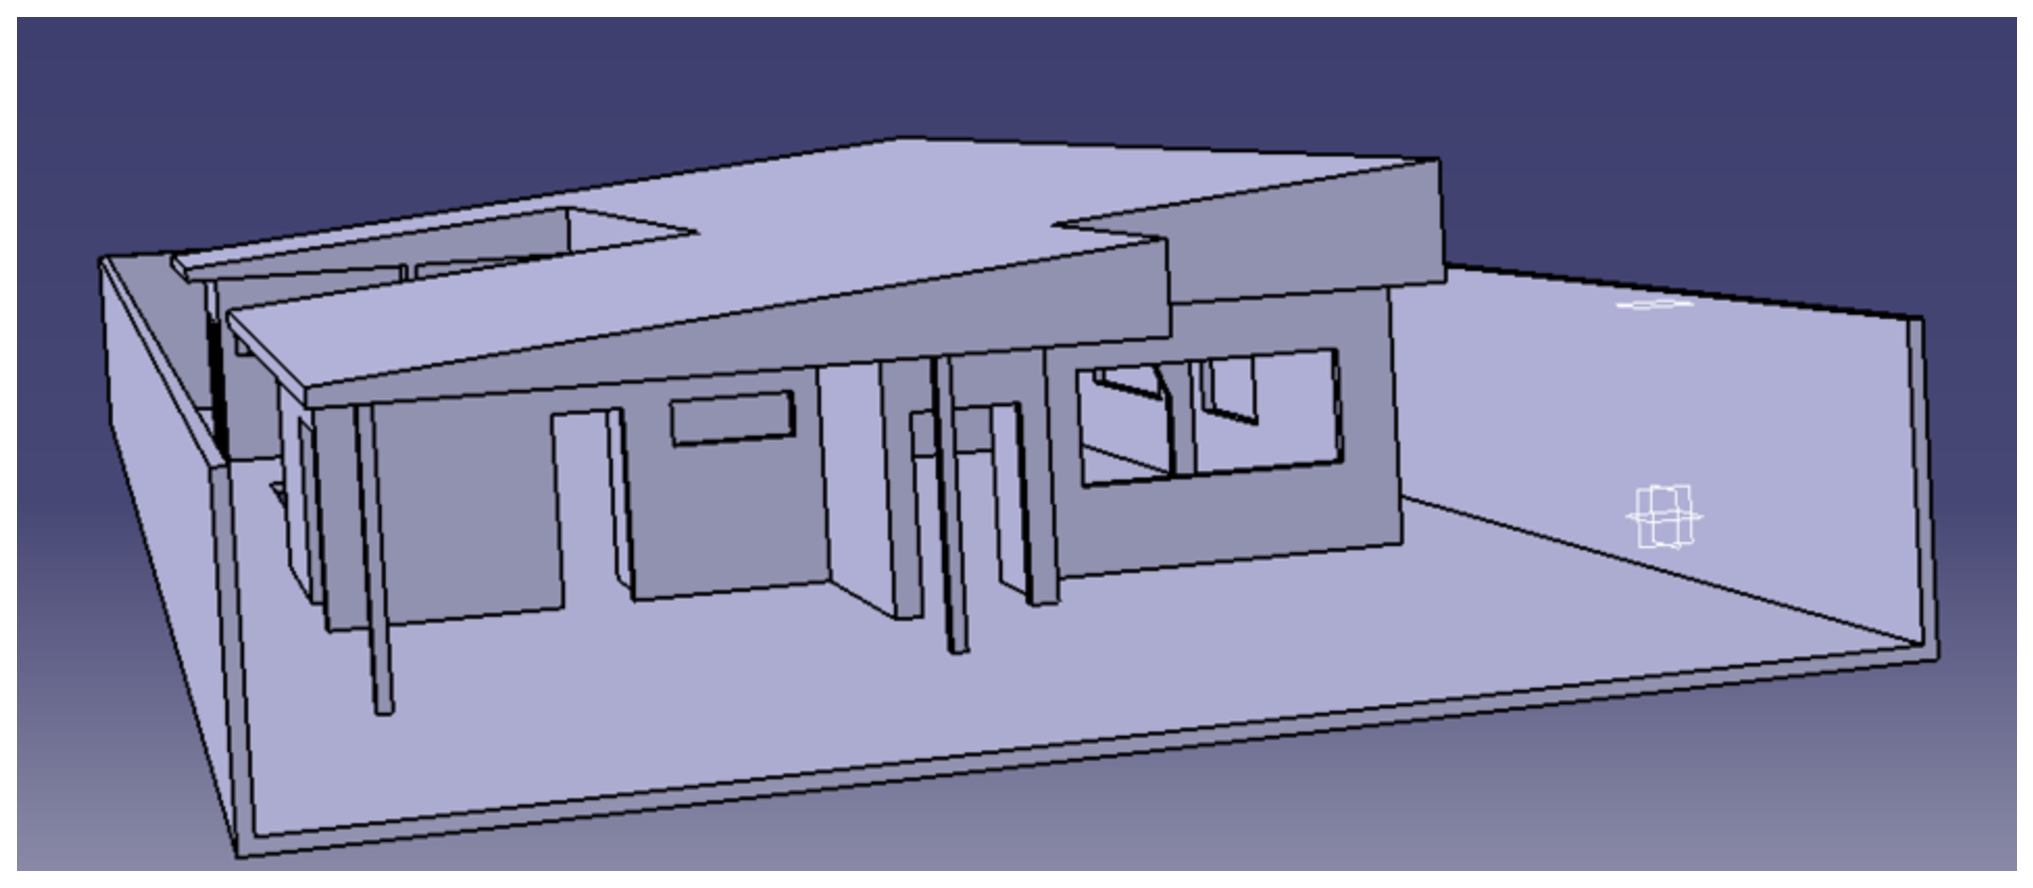
\includegraphics[keepaspectratio,scale=0.5,angle=0]{figuras/3d.eps}
	\caption{Renderização 3D da casa}
  \end{center}
\end{figure}

\subsection{Orçamento da Casa}

	Para o custo direto da casa, que se refere ao total de despesas com insumos, inclusive mão de obra e equipamentos, necessários para a execução da obra \cite{IBEC}, adicionando, neste caso, o preço do terreno, foi necessário adicionar o valor referente aos materiais sustentáveis incluídos no projeto original. Para tanto, considerou-se a seguinte tabela fornecida pelo projetista do projeto com base em valores da SINDUSCON-DF (Sindicado das Indústrias de Construção Civil do Distrito Federal), considerando o padrão de acabamento alto, justificado pelo poder aquisitivo dos moradores, como custo direto original do projeto, totalizando $R\$312.373,42$.  Estimou-se o custo dos materiais tradicionais e o custo dos materiais sustentáveis, assumindo que os outros custos diretos unitários referentes a serviços se mantivessem os mesmos. Subtraindo-se os valor referente aos materiais tradicionais que serão substituidos e adicionando o valor referente aos materiais sustentáveis.

\begin{figure}[H]
  \begin{center}
	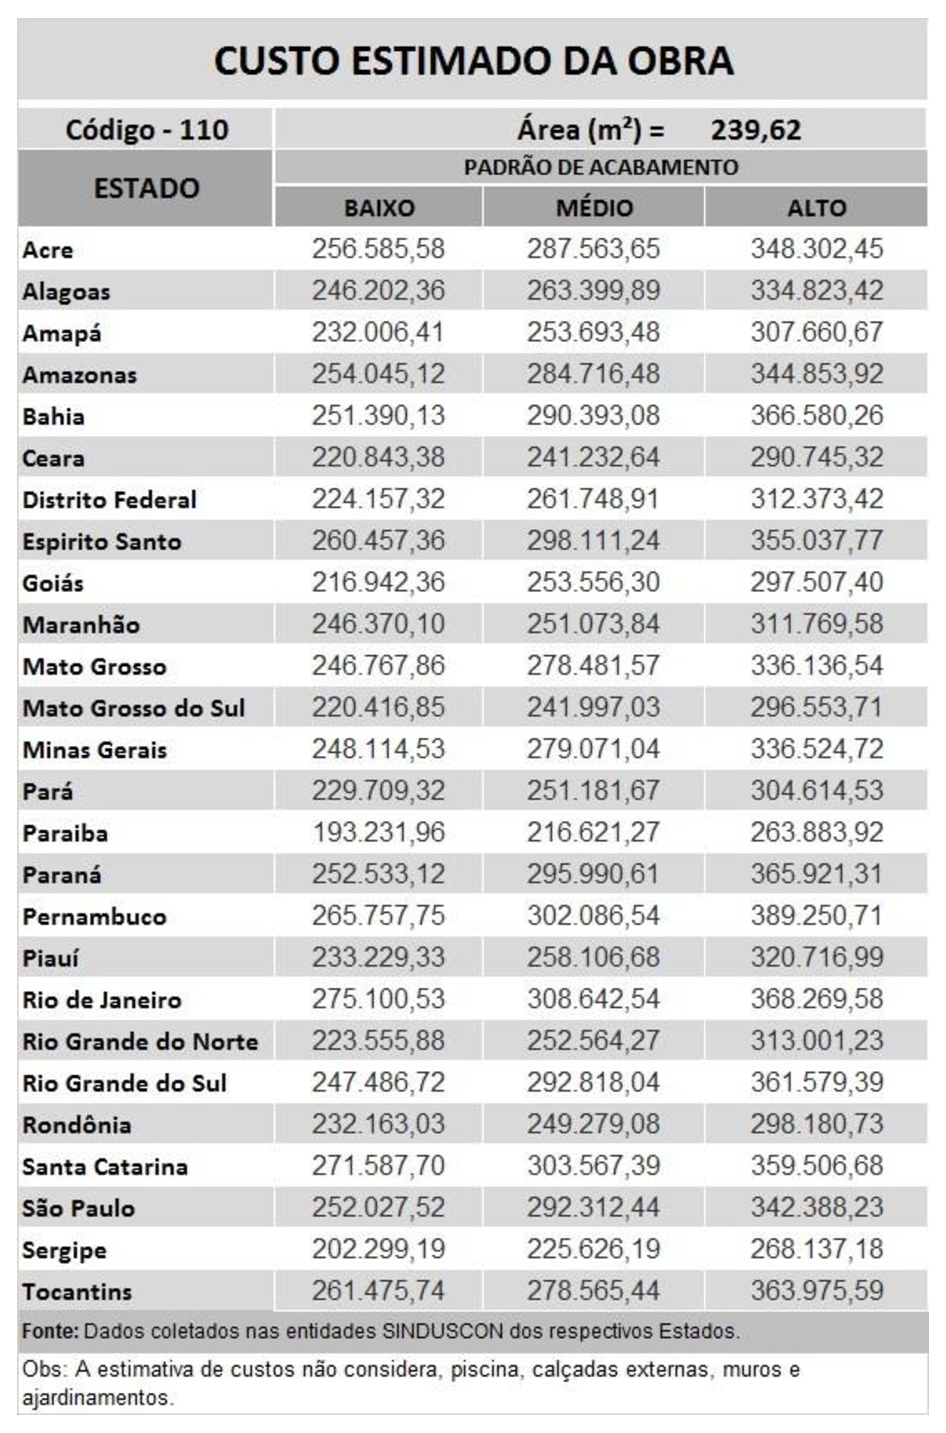
\includegraphics[keepaspectratio,scale=1,angle=0]{figuras/custo_da_obra.eps}
	\caption{Custo estimado da obra}
  \end{center}
\end{figure}

\subsection*{\textbf{Orçamento dos materiais}}

	Para se calcular o orçamento dos materiais foi necessário calcular a quantidade demandada de materiais, para tanto estabeleceu-se área/volume em que cada um seria utilizado e pesquisou-se o preço unitário de cada um, realizando as estimativas de quantidade com base em métodos utilizados na construção civil. Além disso, em cada cálculo da quantidade de materiais adiciona-se uma margem de segurança de 10\% a mais, referente a eventuais perdas de materiais e erros de precisão no cálculo da quantidade, com base em referências de profissionais e sites da área.

\subsubsection*{\textbf{Orçamento dos materiais tradicionais}}

	Com o objetivo de chegar a um valor total estimado da construção da casa, referente aos materiais necessários e o acabamento, foi feito um orçamento no qual se considerou alguns materiais de construção mais utilizados no mercado, que substituiriam os materiais sustentáveis descritos anteriormente.


\subsubsection*{\textbf{Pisos}}

\begin{itemize}

		\item (Internos e externos)Piso Cerâmico - 48 x 48 cm²

		\item Área: 600 m² (Área interna e externa da casa)

		\item Preço: $R\$ 10,90$ a $R\$16,22$

		\item Área ocupada por uma cerâmica: 0,23094 m²

		\item Quantidade necessária: 2604,16 = 2865 cerâmicas

		\item Preço final: $R\$31.228,50$ a $R\$46.470,30$

\end{itemize}

\subsubsection*{\textbf{Paredes}}

\begin{itemize}

		\item Tijolo Cerâmico - 9x19x19 cm [3]

		\item Volume da Parede: 121,338 m³

		\item Superfície da Parede: 425.2155 m²

		\item Consumo do tijolo: 27 peças por m²

		\item Preço: $R\$ 0.59$

		\item Quantidade necessária: 27 * 121.338 = 11481 = 12630 tijolos (+10\%)

		\item Preço final: $R\$7.451,70$
\end{itemize}

\subsubsection*{\textbf{Tinta (Internos e Externos)}}


		\begin{itemize}

		\item Tinta Acrílica - Tintas Universo [4]

		\item Até 55 m² demão/galão, Demãos necessárias: 3

		\item Área: 850,431 m²

		\item Preço unitário: $R\$ 79,90$ (galão com 18 L)

		\item Quantidade necessária: 15,46 = 17 galões

		\item Custo direto unitário: $R\$1.358,30$

\end{itemize}

\subsubsection*{\textbf{Telha}}


\begin{itemize}

		\item Telha Cerâmica Esmaltada - Perkus - 26,50x42x5,50cm [5]

		\item Área: 296,613 m²

		\item Preço unitário: $R\$ 4,09$

		\item Área ocupada por uma telha: 0,1113 m²

		\item Quantidade necessária: 2664,98 = 2931 telhas

		\item Custo direto unitário: $R\$11.987,79$

\end{itemize}


\subsubsection*{\textbf{Madeira}}


\begin{itemize}

		\item Deck Madeira Eucalipto 50X50 Massol

		\item Área: 68,2 m2

		\item Preço unitário: $R\$ 53 ,90$

		\item Área ocupada pelo deck : 0.5 m²

		\item Quantidade necessária : 140 = 154 (+10%)

		\item Adição: Dois bancos de madeira [7]
		
		\item Preço unitário: $R\$ 499,90$

		\item Custo direto unitário: $R\$ 9.300,40$

\end{itemize}

Custo direto relativo aos materiais tradicionais: $R\$ 61.326,69$ a $R\$76.568,49$.

\subsubsection*{\textbf{Orçamento dos materiais sustentáveis}}

\subsubsection*{\textbf{Material: Piso de madeira (Interno)}}


\begin{itemize}

		\item Preço: O preço da ripa de bambu (m²) é de 280,00.

		\item Piso total chão interno da casa: 200 m²

		\item Piso total Banheiro da casa: 17,460 m²
 
		\item Piso total da cozinha: 22,95 m²

		\item Área na qual este tipo de material será usado: 159,590 m² (Todos os cômodos internos, menos cozinha e banheiro)

		\item Número total de ripas: 160 = 176 ripas (+10%)

		\item Custo direto unitário: $R\$49.280,00$

\end{itemize}

\subsubsection*{\textbf{Material: Piso Cerâmico (Externo)}}



\begin{itemize}

		\item Preço: 48x48 cm² está entre $R\$ 27,90$ à $R\$ 34,90$

		\item Área externa da casa: 400 m²

		\item Área dos banheiros: 17,460 m²

		\item Área da cozinha: 22,95 m²

		\item Área total: 440,410 m² (Todas as áreas externas nas quais serão utilizados piso.

		\item Uma cerâmica ocupa: 0,230 m²

		\item Número total de cerâmicas: 1911,501 = 2102 cerâmicas (+10%)

		\item Custo direto unitário: $R\$ 58.645,80$ à $R\$ 73.359,80$

\end{itemize}

\subsubsection*{\textbf{Material: Tijolo Ecológico}}



\begin{itemize}

		\item Preço: Nas medidas de 25cm x 12,5 cm e 7 cm de altura está entre $R\$ 0.92$ à $R\$ 1,20$ a unidade.

		\item Volume total de paredes: 121,338 m³

		\item Volume ocupado por 1 tijolo: $$2,031\times10^{-3} \si{\meter}^{3}$$

		\item Número total de tijolos: 59735,63 = 65709 tijolos (+10\%)

		\item Custo direto unitário: $R\$60.452,00$ à $R\$78.850,80$


\end{itemize}


\subsubsection*{\textbf{Material: Tinta mineral (Internos e externos)}}


\begin{itemize}

		\item Rendimento da pintura: 1LITRO/m²= 18m²/balde, com 2 demãos superfície acabada.

		\item Preço: Balde de 18L = $R\$ 315,00$

		\item Área total das paredes: 850,431 m²

		\item Serão necessários: 47,222 baldes = 53 baldes (+10%)

		\item Custo direto unitário: $R\$ 16.695,00$


\end{itemize}

\subsubsection*{\textbf{Material: Telha}}


\begin{itemize}

		\item Preço unitário: Nas medidas 2,20m x 0,95m x 6mm a partir de $R\$ 45,00$.

		\item Área total telhado: 296,613 m²

		\item Uma telha ocupa: 2,09 m²

		\item Serão necessárias: 141,9 = 157 telhas (+10%)

		\item Custo direto unitário: $R\$7.065,00$

\end{itemize}

\subsubsection*{\textbf{Material: Madeira Plástica}}


\begin{itemize}

		\item Preço: Entre $R\$146,00$ à $R\$ 224,00$ cada metro quadrado, sem a necessidade de manutenção futura.

		\item Área total onde será utilizada : 68,2 m² (No entorno da piscina)

		\item Serão necessários :  68,2 m² = 76,0 m² (+10%)

		\item Adição : Dois bancos de madeira plástica

		\item Preço unitário: $R\$ 334,00$

		\item Custo direto unitário: Entre $R\$ 11.764,00$ a $R\$17.692,00$

\end{itemize}


Somando os custos diretos unitários de cada material sustentável tem-se o total entre $R\$ 203.902,08$ e $R\$ 242.942,60$.

\begin{figure}[H]
  \begin{center}
	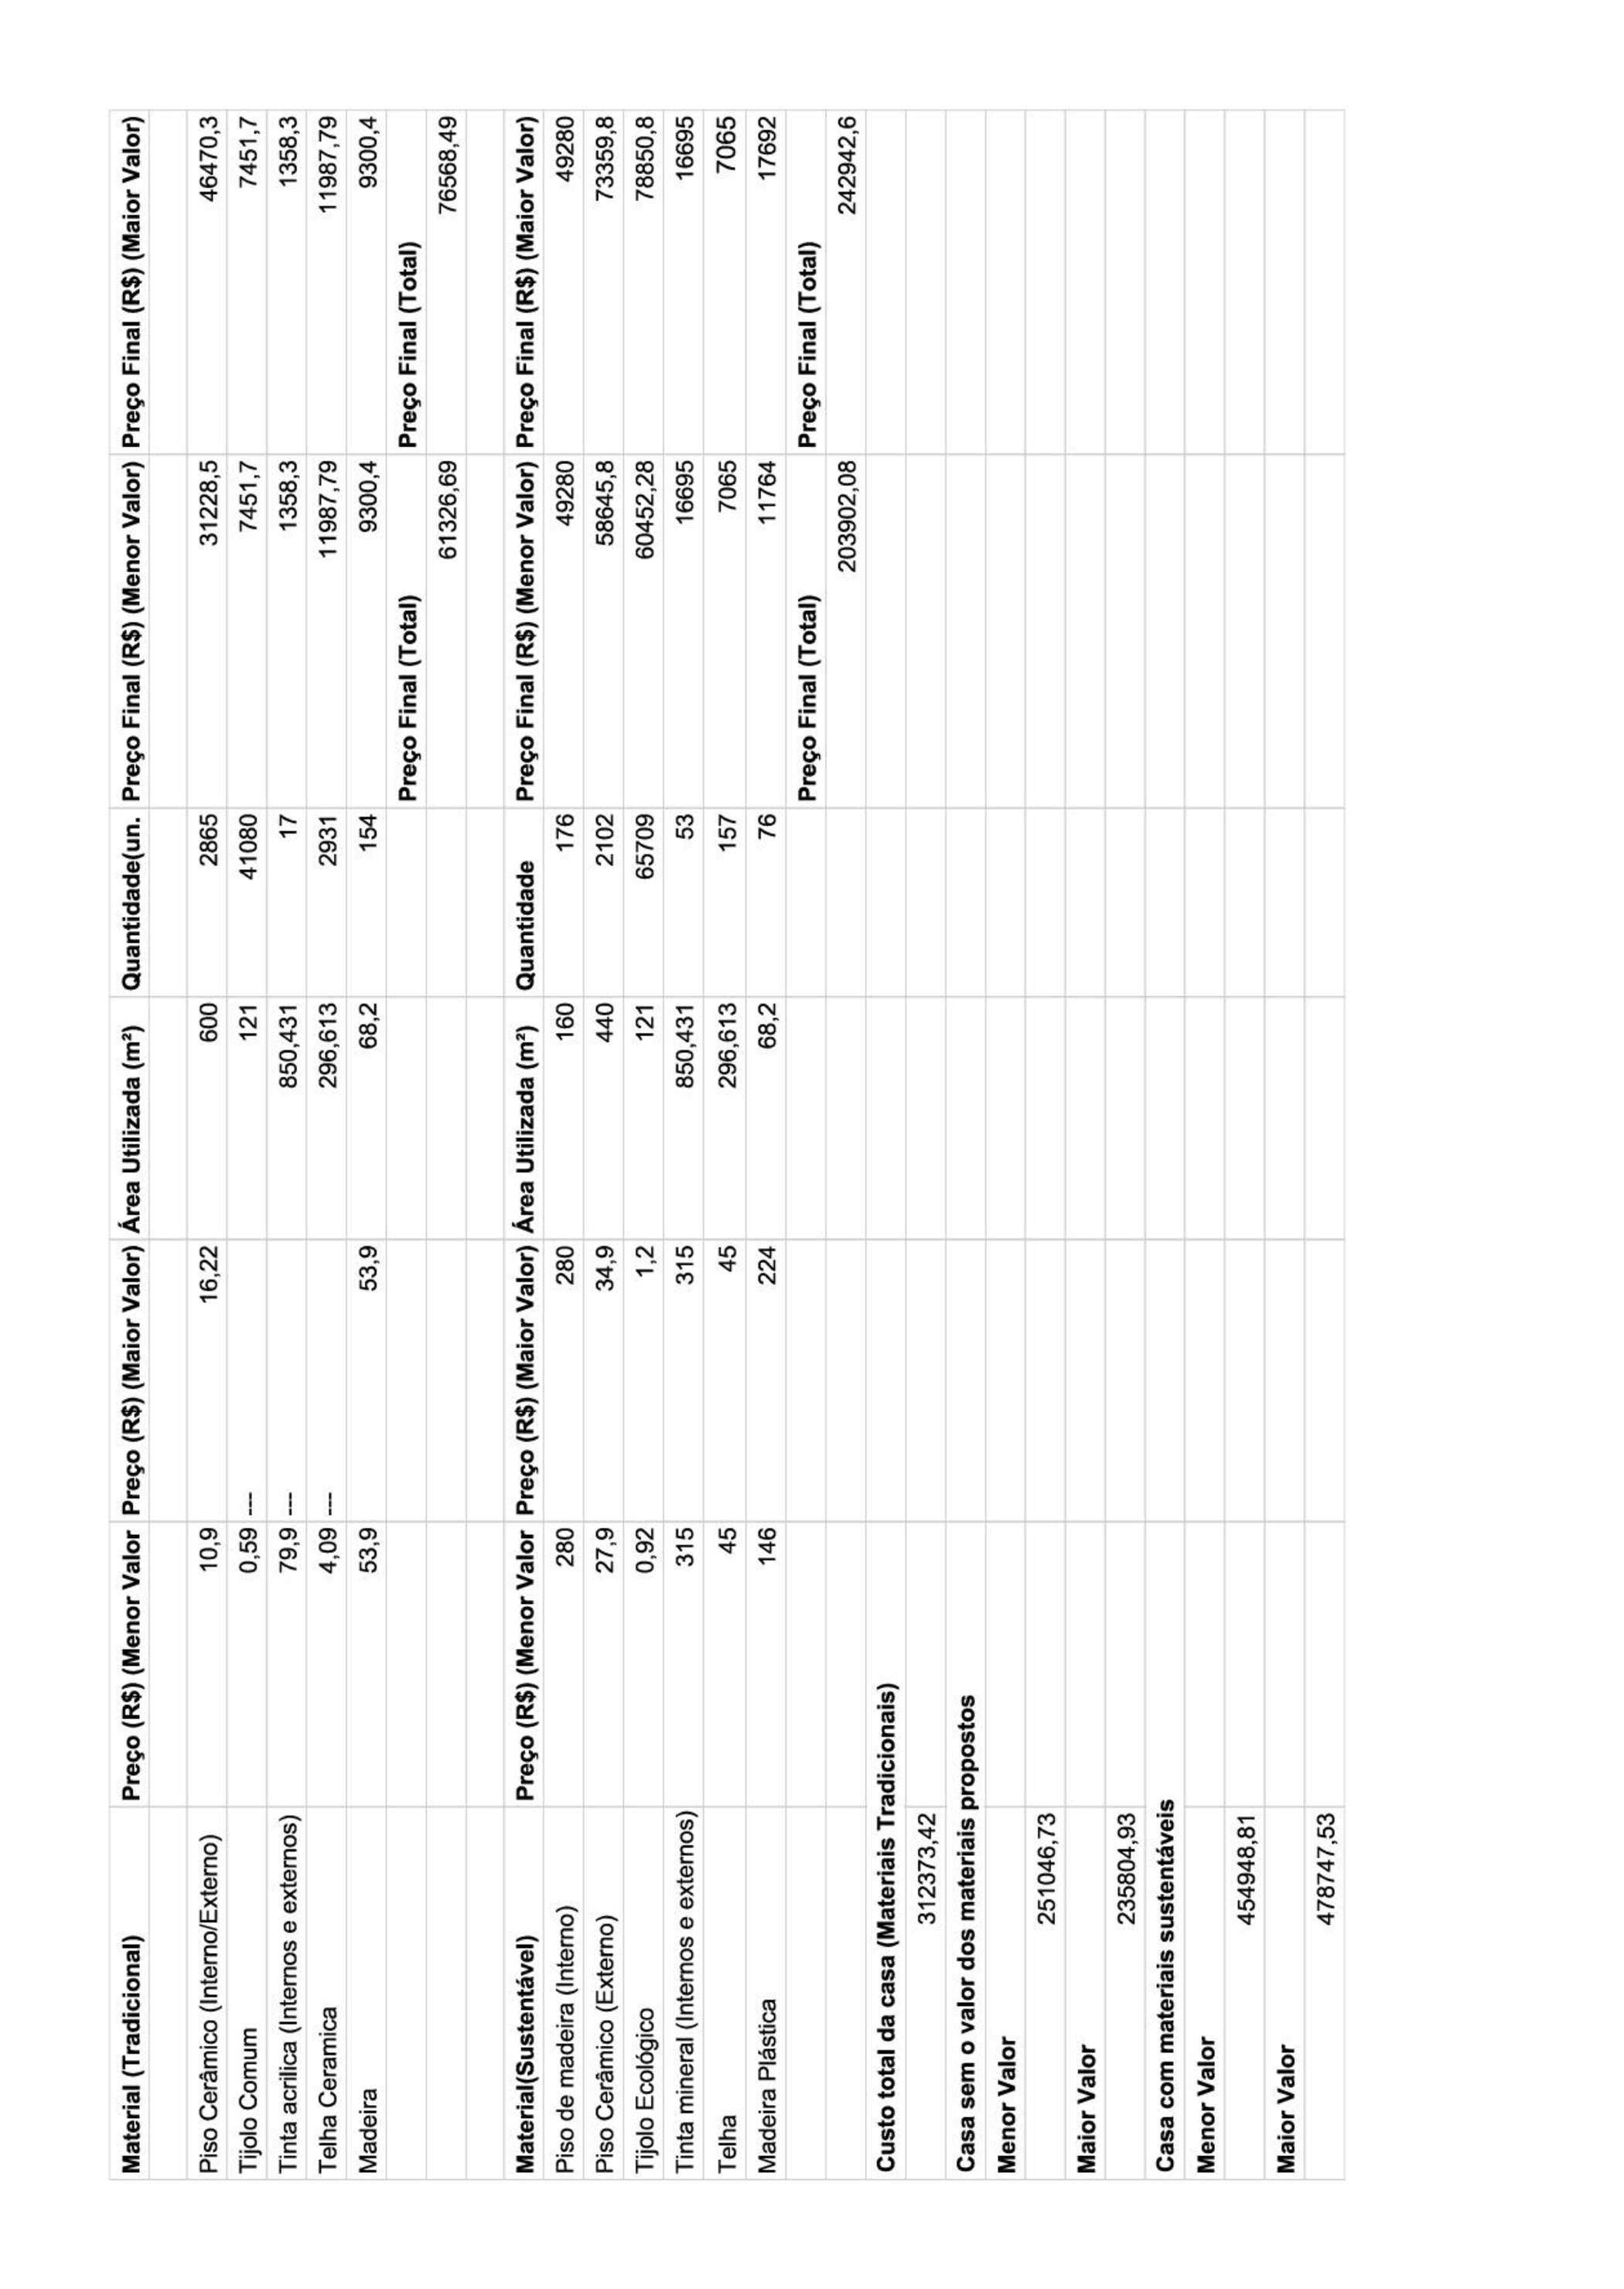
\includegraphics[keepaspectratio,scale=1,angle=0]{figuras/custos_da_casa.eps}
	\caption{Custo estimado da obra}
  \end{center}
\end{figure}
